\section{Teorie grafů}
\label{sec:teorie-grafu}

Velkou část moderní matematiky (zcela jistě topologii, geometrii i algebru)
tvoří studium \uv{struktur}. Toto obecně nedefinované slovo obvykle značí
množinu s nějakou další informací o vztahu mezi jejími prvky -- tím obvykle bývá
operace nebo třeba, jako v případě grafů, relace.

Tato kapitola zároveň značí jakýsi milník ve vývoji matematického myšlení,
především algebraickým směrem. Můžeme se totiž začít bavit o speciálních
zobrazeních, které zachovávají strukturu na množinách, mezi kterými vedou, tzv.
\emph{homomorfismech}; pochopit, že je dobré mít více popisů stejné struktury
ekvivalentních v tom smyslu, že poskytují stejné množství informací, přestože se
o žádné bijekci nedá formálně hovořit; uvidět, že je užitečné dva různé grafy
(či obecně dvě různé struktury) považovat za stejné, když se liší pouze
zanedbatelně.

Jednou, avšak zdaleka ne \emph{jedinou}, motivací pro teorii grafů je schopnost
analyzovat struktury tvořené množinou \uv{uzlů}, mezi některýmiž vedou
\uv{spojnice}. Takováto struktura úspěšně modeluje až neuvěřitelné množství
přírodních i společenských úkazů. Mezi nimi jmenujmež
\begin{itemize}
 \item návrhy elektrických obvodů, kde uzly jsou elektrická zařízení a spojnice
  jsou kabely mezi nimi vedoucí;
 \item lingvistické modely, kde uzly jsou slova a spojnice vede mezi
  těmi syntakticky souvisejícími;
 \item studium molekul, kde uzly jsou atomy a spojnice vazby mezi nimi;
 \item analýza šíření fámy v sociologii, kde uzly jsou lidské komunity a
  spojnice vede mezi komunitami s bezprostředním kontaktem.
\end{itemize}

Snad pro to, že uzly a spojnice grafu se obvykle kreslí jako body a úsečky
v~prostoru, ujaly se pro ně názvy \emph{vrcholy} a \emph{hrany} (jako v
mnohoúhelnících), respektive. Struktura zvaná \emph{graf} tedy sestává ze dvou
údajů:
\begin{enumerate}
 \item množiny (obvykle konečné) vrcholů značené $V$ a
 \item množiny hran $E$, která je spjata s množinou vrcholů; toto \uv{sepětí} se
  však definuje různě, v závislosti na vkusu a aplikaci. My si ukážeme tři z
  jistě většího množství různých definic.
\end{enumerate}

Asi prvním přirozeným kandidátem pro \uv{strukturu} je množina s relací. To je
také první způsob, jak si budeme definovat pojem \emph{graf}. Je to také ten
nejobecnější v tom smyslu, že jeho pouze drobné modifikace nám umožní definovat
i obdobné struktury, jež také zmateně slují \emph{grafy}, byť s připojeným
atributem.

Abychom úsečky mezi body mohli popsat jako relaci, čili pomocí uspořádaných
dvojic bodů, zcela jistě budeme požadovat, aby nevedly úsečky z~bodu do něho
samého. Úsečku délky $0$ lze totiž triviálně ztotožnit s bodem. Dále, úsečka z
bodu $A$ do bodu $B$ je jistě tatáž, kterak úsečka z bodu $B$ do bodu $A$. Tento
fakt musí rovněž relace $E$ odrážet.

První vlastností relace se, snad nepřekvapivě, říká \emph{antireflexivita}.
Čili, relace $E$ na $V$ je \emph{antireflexivní}, když hrana $(v,v) \notin E$
pro každý vrchol $v \in V$.

Druhou vlastnost už jsme potkali a nazvali ji symetrií. Požadujeme, aby s~hranou
$(v,w) \in E$ obsahovala $E$ též hranu $(w,v) \in E$ pro každé dva vrcholy $v,w
\in V$.

\begin{definition}[Graf poprvé]
\label{def:graf-poprve}
 Dvojici $G \coloneqq (V,E)$, kde $V$ je konečná množina a $E$ je relace na $V$,
 nazveme \emph{grafem}, pokud je $E$ \textbf{antireflexivní} a
 \textbf{symetrická}.
\end{definition}

\begin{remark}
 Z hlediska ryze formálního neodpovídá tato definice dokonale naší geometrické
 představě. My jsme totiž pouze požadovali, aby $E$ obsahovala jak úsečku z $v$ 
 do $w$, tak úsečku z $w$ do $v$, ale nikoli, aby se jednalo o \emph{tutéž}
 úsečku. Tedy, jedna úsečka mezi body je v~množině $E$ reprezentována dvěma
 dvojicemi.

 Nápravou by bylo definovat navíc ještě relaci $R$ na $E$, kde $(v,v')$ je
 v~relaci $R$ s $(w,w')$ právě tehdy, když $(w,w') = (v',v)$ nebo $(w,w') =
 (v,v')$. Jinak řečeno, úsečka z bodu $v$ do bodu $v'$ je v relaci sama se sebou
 a s úsečkou z bodu $v'$ do bodu $v$.

 Uvážíme-li pak jako hrany grafu $G$ nikoli množinu $E$, ale její třídy
 ekvivalence podle $R$ (\textbf{Ověřte, že $R$ je ekvivalence!}), dostaneme již
 přesnou množinovou paralelu bodů a úseček.

 My však budeme v zájmu přehlednosti tento nedostatek ignorovat, protože není
 pro pochopení ani rozvoj teorie relevantní.
\end{remark}

Cesta k druhé možné definici grafu není od první daleká. Stačí vlastně relaci
$E$ interpretovat trochu jinak. Přece, antireflexivní a symetrická relace je
\uv{totéž} jako množina dvouprvkových podmnožin $V$.

Vskutku, vezměme nějakou $E' \subseteq \binom{V}{2}$. Relaci $E$ z
\myref{definice}{def:graf-poprve} sestrojíme tak, že z množiny $\{v,w\} \in E'$
vyrobíme dvojice $(v,w)$ a $(w,v)$. Protože prvky v množině nejsou uspořádané a
nemohou se opakovat, dává tato konstrukce opravdu antireflexivní a symetrickou
relaci. Vizuálně odpovídá rozdělení úsečky mezi $v$ a $w$ na šipku z $v$ do $w$
a šipku z $w$ do $v$.

Z druhé strany, mějme nějakou antireflexivní a symetrickou relaci $E$ na $V$.
Protože s dvojicí $(v,w)$ obsahuje $E$ i dvojici $(w,v)$, můžeme z těchto dvojic
ztvárnit množinu $\{v,w\}$. Relace $E$ je antireflexivní, čili se nemůže stát,
že $v = w$, a množina $\{v,w\}$ je pročež vždy dvouprvková. Posbíráme-li všechny
množiny $\{v,w\}$ do jedné velké množiny $E'$, bude platit $E' \subseteq
\binom{V}{2}$. Vizuálně odpovídá tato konstrukce slepení šipky z $v$ do $w$ a
šipky z $w$ do $v$ do jedné úsečky mezi $v$ a $w$.

\begin{warning}
 Mezi množinami $E$ a $E'$ \textbf{nemůže existovat bijekce}, třeba jen pro to,
 že $\# E = 2 \# E'$. Co konstrukce v předchozích dvou odstavcích ukazují, je
 pouze fakt, že pro naše účely definují $E$ a $E'$ stejnou strukturu na množině
 $V$.

 Ovšem, uvážili-li bychom místo $E$ pouze třídy ekvivalence jejích prvků podle
 relace $R$ popsané v poznámce pod \myref{definicí}{def:graf-poprve}, pak bychom
 skutečně tímto způsobem našli bijekci s množinou $E'$.
\end{warning}

\begin{definition}[Graf podruhé]
\label{def:graf-podruhe}
 Dvojici $G \coloneqq (V,E')$, kde $V$ je konečná množina a $E' \subseteq
 \binom{V}{2}$, nazveme \emph{grafem}.
\end{definition}

Třetí pohled na hrany v grafu je více \uv{kategoriální}. Zatímco množiny $E$ a
$E'$ jsou závislé ve své definici na množině $V$, třetí množina hran $E''$,
kterou si zde definujeme, bude libovolná konečná množina.

Tento popis grafové struktury bude odpovídat trochu jiné představě; konkrétně
takové, kdy začínáme s množinou bodů $V$ a s množinou šipek $E$ (jež jsou od
sebe naprosto odděleny) a oba konce každé šipky zapíchneme do dvou různých bodů
z $V$. Toto \uv{zapíchnutí} realizují zobrazení $s,t: E'' \to V$ (z angl.
\textbf{s}ource a \textbf{t}arget), která zobrazují šipky z $E''$ do bodů z $V$.
Přičemž budeme trvat na tom, aby $s(e) \neq t(e)$ pro všechny šipky $e \in E''$
a navíc, aby pro každou $e \in E''$ existovala šipka $e' \in E''$ taková, že
$s(e) = t(e')$, $t(e) = s(e')$. Lidsky řečeno, nesmíme zapíchnout konce šipky do
téhož vrcholu a, když zapíchneme začátek šipky do bodu $v$ a její konec do bodu
$w$, pak musíme vzít další šipku, jejíž začátek zapíchneme do $w$ a konec do
$v$.

Je snadné si rozmyslet, že z množiny šipek $E''$ zrekonstruujeme množinu $E$ z
\myref{definice}{def:graf-poprve} tak, že z šipky $e \in E''$ vytvoříme dvojici
$(s(e),t(e)) \in E$. Podmínky kladené na zobrazení $s$ a $t$ zaručují, že
vzniklá množina $E$ je relace na $V$, která je antireflexivní a symetrická. V
tomto případě dává uvedená konstrukce dokonce bijekci $E \cong E''$, čili jsme
opět definovali tutéž strukturu na $V$.

Tato struktura bude zvlášť užitečná, až budeme probírat \emph{toky v síti}.

\begin{definition}[Graf potřetí]
\label{def:graf-potreti}
 Čtveřici $G \coloneqq (V,E'',s,t)$, kde $V$ a $E''$ jsou konečné množiny a $s$ 
 a $t$ jsou zobrazení $E'' \to V$ nazveme \emph{grafem}, pokud
 \begin{enumerate}[label=(\alph*)]
  \item $s(e) \neq t(e) \; \forall e \in E''$ a
  \item $\forall e \in E'' \; \exists e' \in E'': s(e) = t(e') \wedge t(e) =
   s(e')$.
 \end{enumerate}
\end{definition}

\begin{remark}
 Opět, aby \myref{definice}{def:graf-potreti} odpovídala představě bodů a
 úseček (nebo oboustranných šipek), museli bychom definovat relaci $R$ na $E$
 tak, aby $e$ a $e'$ byly v $R$, právě když $s(e) = s(e')$ a $t(e) = t(e')$ nebo
 $s(e) = t(e')$ a $t(e) = s(e')$. V takovém případě bychom mohli sestrojit
 bijekci mezi $E''$ a $E'$ z \myref{definice}{def:graf-podruhe}.
\end{remark}

\begin{example}
 \label{exam:interpretace-grafu}
 Ať $V \coloneqq \{1,2,3,4,5\}$ a 
 \begin{enumerate}
  \item $E \coloneqq
   \{(1,2),(2,1),(1,3),(3,1),(1,4),(4,1),(1,5),(5,1),(2,3),(3,2),\\(4,5),(5,4)\}$;
  \item $E' \coloneqq \{\{1,2\},\{1,3\},\{1,4\},\{1,5\},\{2,3\},\{4,5\}\}$;
  \item $E'' \coloneqq
   \{e_1,e_2,e_3,e_4,e_5,e_6,e_1',e_2',e_3',e_4',e_5',e_6'\}$, kde
   \begin{enumerate}
    \item $s(e_1) = s(e_2) = s(e_3) = s(e_4) = 1$, $s(e_5) = 2$, $s(e_6) = 4$,
    \item $t(e_1) = 2$, $t(e_2) = t(e_5) = 3$, $t(e_3) = 4$, $t(e_4) = t(e_6) =
     5$ a
    \item $(s(e_i),t(e_i)) = (t(e_i'),s(e_i'))$ pro všechna $i \leq 6$.
   \end{enumerate}
 \end{enumerate}

 Není těžké nahlédnout, že $E$, $E'$ i $(E'',s,t)$ definují tutéž strukturu na
 $V$. Nakreslíme si grafy $G = (V,E), G' = (V,E')$ a $G'' = (V,E'',s,t)$.
 Přičemž hrany z $E$ budeme kreslit jako oboustranné šipky, ty z $E'$ jako
 prosté úsečky a ty z $E''$ rozdělíme na dvě protichůdné šipky, abychom
 vyjádřili rozdíly v interpretaci těchto grafových struktur.

 Graf $G = (V,E)$ vypadá například \hyperref[fig:graf-poprve]{takto}. Pomněte,
 že například oboustranná šipka mezi vrcholy $1$ a $2$ představuje ve
 skutečnosti \textbf{dvě} dvojice -- $(1,2)$ a $(2,1)$ z relace $E$.
 \begin{figure}[H]
  \centering
  \begin{tikzpicture}[scale=1.5]
   \tikzset{vertex/.style = {shape=circle,draw,minimum size=1.5em,inner sep=1pt}}
   \tikzset{edge/.style = {<->,>={Latex[length=2.5mm]}}}
   \node[vertex] (1) at (0, 0) {$1$};
   \node[vertex] (2) at (-2, 1) {$2$};
   \node[vertex] (3) at (-2, -1) {$3$};
   \node[vertex] (4) at (2, 1) {$4$};
   \node[vertex] (5) at (2, -1) {$5$};

   \draw[edge,thick] (1) -- (2)
   node[above right=2.5mm and 1mm,midway,rotate=-26,anchor=mid]{$(2,1)$}
   node[below left=3mm and 1.5mm,midway,rotate=-26,anchor=mid]{$(1,2)$};
   \draw[edge,thick] (1) -- (3)
   node[above left=2.5mm and 1mm,midway,rotate=26,anchor=mid]{$(3,1)$}
   node[below right=3mm and 1.5mm,midway,rotate=26,anchor=mid]{$(1,3)$};
   \draw[edge,thick] (1) -- (4)
   node[above left=2.5mm and 1mm,midway,rotate=26,anchor=mid]{$(1,4)$}
   node[below right=3mm and 1.5mm,midway,rotate=26,anchor=mid]{$(4,1)$};
   \draw[edge,thick] (1) -- (5)
   node[above right=2.5mm and 1mm,midway,rotate=-26,anchor=mid]{$(1,5)$}
   node[below left=3mm and 1.5mm,midway,rotate=-26,anchor=mid]{$(5,1)$};
   \draw[edge,thick] (2) -- (3)
   node[left=3mm,rotate=-90,midway,anchor=mid]{$(3,2)$}
   node[right=3mm,rotate=-90,midway,anchor=mid]{$(2,3)$};
   \draw[edge,thick] (4) -- (5)
   node[left=3mm,rotate=-90,midway,anchor=mid]{$(5,4)$}
   node[right=3mm,rotate=-90,midway,anchor=mid]{$(4,5)$};
  \end{tikzpicture}
  \caption{Graf jako množina $V$ s relací $E$.}
  \label{fig:graf-poprve}
 \end{figure}

 Zcela stejně vypadá i graf $G' = (V,E')$.
 \begin{figure}[H]
  \centering
  \begin{tikzpicture}[scale=1.5]
   \tikzset{vertex/.style = {shape=circle,draw,minimum size=1.5em,inner sep=1pt}}
   \node[vertex] (1) at (0, 0) {$1$};
   \node[vertex] (2) at (-2, 1) {$2$};
   \node[vertex] (3) at (-2, -1) {$3$};
   \node[vertex] (4) at (2, 1) {$4$};
   \node[vertex] (5) at (2, -1) {$5$};

   \draw[thick] (1) -- (2)
   node[above right=2.5mm and 1mm,midway,rotate=-26,anchor=mid]{$\{1,2\}$};
   \draw[thick] (1) -- (3)
   node[above left=2.5mm and 1mm,midway,rotate=26,anchor=mid]{$\{1,3\}$};
   \draw[thick] (1) -- (4)
   node[above left=2.5mm and 1mm,midway,rotate=26,anchor=mid]{$\{1,4\}$};
   \draw[thick] (1) -- (5)
   node[above right=2.5mm and 1mm,midway,rotate=-26,anchor=mid]{$\{1,5\}$};
   \draw[thick] (2) -- (3)
   node[right=3mm,rotate=-90,midway,anchor=mid]{$\{2,3\}$};
   \draw[thick] (4) -- (5)
   node[right=3mm,rotate=-90,midway,anchor=mid]{$\{4,5\}$};
  \end{tikzpicture}
  \caption{Graf jako množiny $V$ a $E' \subseteq \binom{V}{2}$.}
  \label{fig:graf-podruhe}
 \end{figure}

 Konečně, $G'' = (V,E'',s,t)$ můžeme načrtnout taktéž velmi podobně.
 \begin{figure}[H]
  \centering
  \begin{tikzpicture}[scale=1.5]
   \tikzset{vertex/.style = {shape=circle,draw,minimum size=1.5em,inner sep=1pt}}
   \tikzset{edge/.style = {->,>={Latex[length=2.5mm]}}}
   \node[vertex] (1) at (0, 0) {$1$};
   \node[vertex] (2) at (-2, 1) {$2$};
   \node[vertex] (3) at (-2, -1) {$3$};
   \node[vertex] (4) at (2, 1) {$4$};
   \node[vertex] (5) at (2, -1) {$5$};

   \draw[edge,thick,transform canvas={yshift=1mm,xshift=1mm},shorten <=-2pt] (2) -- (1)
   node[above right=2.5mm and 1mm,midway,rotate=-26,anchor=mid]{$e_1$};
   \draw[edge,thick,transform canvas={yshift=-1mm,xshift=-1mm},shorten <=-2pt] (1) -- (2)
   node[below left=2.5mm and 1.5mm,midway,rotate=-26,anchor=mid]{$e'_1$};

   \draw[edge,thick,transform canvas={yshift=1mm,xshift=-1mm},shorten >=-2pt] (3)
   -- (1)
   node[above left=3mm and 1mm,midway,rotate=26,anchor=mid]{$e'_2$};
   \draw[edge,thick,transform canvas={yshift=-1mm,xshift=1mm},shorten >=-2pt] (1)
   -- (3)
   node[below right=2.5mm and 1.5mm,midway,rotate=26,anchor=mid]{$e_2$};

   \draw[edge,thick,transform canvas={yshift=1mm,xshift=-1mm},shorten >=-2pt] (1)
   -- (4)
   node[above left=3mm and 1mm,midway,rotate=26,anchor=mid]{$e_3$};
   \draw[edge,thick,transform canvas={yshift=-1mm,xshift=1mm},shorten >=-2pt] (4)
   -- (1)
   node[below right=2.5mm and 1.5mm,midway,rotate=26,anchor=mid]{$e'_3$};

   \draw[edge,thick,transform canvas={yshift=1mm,xshift=1mm},shorten <=-2pt] (1)
   -- (5)
   node[above right=2.5mm and 1mm,midway,rotate=-26,anchor=mid]{$e_4$};
   \draw[edge,thick,transform canvas={yshift=-1mm,xshift=-1mm},shorten <=-2pt]
   (5) -- (1)
   node[below left=2.5mm and 1.5mm,midway,rotate=-26,anchor=mid]{$e'_4$};

   \draw[edge,thick,transform canvas={xshift=1mm},shorten >=-2pt] (2)
   -- (3)
   node[right=3mm,rotate=-90,midway,anchor=mid]{$e_5$};
   \draw[edge,thick,transform canvas={xshift=-1mm},shorten >=-2pt] (3)
   -- (2)
   node[left=3mm,rotate=-90,midway,anchor=mid]{$e'_5$};

    \draw[edge,thick,transform canvas={xshift=1mm},shorten >=-2pt] (4)
   -- (5)
   node[right=3mm,rotate=-90,midway,anchor=mid]{$e_6$};
   \draw[edge,thick,transform canvas={xshift=-1mm},shorten >=-2pt] (5)
   -- (4)
   node[left=3mm,rotate=-90,midway,anchor=mid]{$e'_6$};
  \end{tikzpicture}
  \caption{Graf jako množina $V$ s trojicí $(E'',s,t)$.}
  \label{fig:graf-potreti}
 \end{figure}
\end{example}

\begin{warning}
 Grafová struktura je obecně zcela nezávislá na jejím nakreslení. Například graf
 $G = (V,E')$ z \hyperref[exam:interpretace-grafu]{předchozího příkladu} lze
 ekvivalentně vyobrazit třeba následovně.
 \begin{figure}[H]
  \centering
  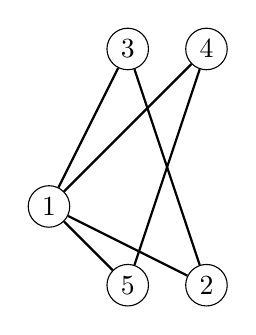
\begin{tikzpicture}
   \tikzset{vertex/.style = {shape=circle,draw,minimum size=1.5em,inner sep=1pt}}
   \node[vertex] (1) at (0, -1) {$1$};
   \node[vertex] (2) at (2, -2) {$2$};
   \node[vertex] (3) at (1, 1) {$3$};
   \node[vertex] (4) at (2, 1) {$4$};
   \node[vertex] (5) at (1, -2) {$5$};

   \draw[thick] (1) -- (2);
   \draw[thick] (1) -- (3);
   \draw[thick] (1) -- (4);
   \draw[thick] (1) -- (5);
   \draw[thick] (2) -- (3);
   \draw[thick] (4) -- (5);
  \end{tikzpicture}
  \caption{Graf $G = (V,E')$ nakreslený jinak.}
  \label{fig:graf-podruhe}
 \end{figure}

\end{warning}

V následujícím textu spojíme všechny tři interpretace dohromady a pro $v,w \in
V$ budeme hranu mezi $v$ a $w$ značit zjednodušeně jako $vw$. Pokud nehrozí
nedorozumění, budeme pod tímto zápisem rozumět hranu, jejíž začátek je $v$ a
konec $w$, čili $s(vw) = v$ a $t(vw) = w$. Avšak, kdykoli se nám to bude hodit,
ztotožníme ji bez okolků s hranou $wv$ s obrácenými konci.

Tento neformální přístup k popisu hran se může zdát jako nebezpečný, ale jak
uvidíme, ve skutečnosti velmi zjednodušuje zápis a újma na rigorozitě je obecně
minimální. Kompletněji řečeno, hranou mezi dvěma vrcholy ${v,w \in V}$ myslíme
buď dvojici $(v,w) \in E$ nebo dvojici $(w,v) \in E$ nebo množinu $\{v,w\} \in
E'$ nebo prvek $e \in E''$ takový, že $s(e) = v$ a $t(e) = w$, nebo prvek $e'
\in E''$ takový, že $s(e') = w$ a $t(e') = v$, a je nám to u ...

Obecně, v teorii grafů se velmi často pracuje s konečnými posloupnostmi (či
$n$-ticemi, chcete-li) vrcholů a hran. Zavedeme proto zjednodušené značení
$x_1x_2\cdots x_n$ pro uspořádanou $n$-tici $(x_1,\ldots,x_n)$. Kdyby hrozil
konflikt se zápisem součinu prvků $x_1,\ldots,x_n$, samozřejmě tento úzus
dočasně opustíme.

\begin{exercise}
 Nakreslete graf $G = (V,E)$, kde
 \begin{itemize}
  \item $V = \{1,\ldots,5\}, E = \{\{1,2\}, \{1,3\}, \{1,5\}, \{2,3\},
   \{3,4\},\{4,5\}\}$.
  \item $V = \{1,\ldots,5\}$, $E = \binom{V}{2}$.
  \item $V = \{1,\ldots,8\}$, $E = \{e_1,\ldots,e_8\}$ a
  \begin{itemize}
   \item $t(e_i) = s(e_{i+1}) = i + 1$ pro všechna $i \leq 7$,
   \item $t(e_8) = s(e_1) = 1$.
  \end{itemize}
 \end{itemize}
\end{exercise}

\begin{exercise}
 Popište všechny grafy $G = (V,E)$, kde $E$ je relace na $V$, která je
 antireflexivní, symetrická (to je součástí definice grafu) a navíc
 \textbf{transitivní}.
\end{exercise}

\begin{exercise}
 Ať $V$ je konečná množina a $E$ je relace na $V$, která je antireflexivní a
 symetrická. Definujme navíc na $E$ další relaci $ \sim $ předpisem
 \[
  (v,v') \sim (w,w') \Leftrightarrow (v,v') = (w,w') \vee (v,v') = (w',w). 
 \]
 Dokažte, že pak existuje bijekce mezi $[E]_{ \sim }$ a množinou
 \[
  E' \coloneqq \{\{v,v'\} \mid (v,v') \in E\},
 \]
 čili mezi množinou tříd ekvivalence $E$ podle $ \sim $ a množinou, kterou
 dostanu tak, že z uspořádaných dvojic v $E$ udělám neuspořádané dvojice, tj.
 dvouprvkové podmnožiny. Pro intuici vizte poznámku pod
 \myref{definicí}{def:graf-poprve}.
\end{exercise}

\begin{exercise}
 Spočtěte, kolik existuje grafů na $n$ vrcholech.
\end{exercise}

\subsection{Pohyb v grafu}
\label{ssec:pohyb-v-grafu}

Jak jsme zmínili na začátku kapitoly, mnoho aplikací teorie grafů využívá
interpretace této struktury jako množiny \uv{uzlů} se \uv{spojnicemi}, po
kterých se dá mezi uzly pohybovat. V této podsekci dáme pohybu po spojnicích
formální tvář.

Nejzákladnějším typem pohybu v grafu je libovolná posloupnost vrcholů se zcela
přirozenou podmínkou, že mezi vrcholy v posloupnosti bezprostředně za sebou musí
vést hrana. Takové posloupnosti se říká \emph{sled} (angl. \emph{walk}).

\begin{definition}[Sled poprvé]
\label{def:sled-poprve}
 Ať $G = (V,E)$ je graf. Posloupnost vrcholů $v_1v_2\cdots v_n$ nazveme
 \emph{sledem} v grafu $G$, pokud $v_i v_{i+1} \in E$ pro každý index ${i \in
 \{1,\ldots,n-1\}}$.
\end{definition}

Je však užitečné si uvědomit, že každý sled lze ekvivalentně definovat jako
posloupnost navazujících hran. Tento pohled (jak uvidíme později v kapitole) má
své aplikace -- často nás totiž zajímá, po kterých spojnicích chodíme, spíše než
které uzly procházíme.

Máme-li sled $v_1v_2 \cdots v_n$, tak každá dvojice $v_iv_{i+1}$ musí být hranou
v $G$. To ovšem znamená, že zcela identickou informaci poskytuje i posloupnost
hran $e_1e_2 \cdots e_{n-1}$, kde $e_i = v_iv_{i+1}$.

\begin{remark}
 Tento princip, který prostupuje matematické struktury, je až překvapivě
 zásadního významu. Zobecníme-li trochu předchozí pozorování, uvědomíme si, že
 množina hran vlastně už v sobě obsahuje informaci o všech prvcích množiny $V$.
 Tedy bychom dokonce mohli definovat graf pouze jako množinu hran a množinu
 vrcholů bychom takto získali automaticky. Opak samozřejmě není pravdou.

 Situace, kdy struktura na množině (či něčem složitějším) je dostatečně
 \uv{hustá}, aby obsahovala kompletní informaci o této množině, je obecně velmi
 žádaná, jelikož struktura je často konstruována systematicky (a tedy jí
 rozumíme lépe) ve srovnání s náhodnou volbou její bázové množiny.

 Pro nedostatek představivosti uvedeme příklad z homologické algebry, kde
 injektivní a projektivní rezolventy modulů obsahují již kompletní informaci o
 daném modulu. Tedy člověku pro pochopení teorie modulů z homologického hlediska
 \uv{stačí} studovat injektivní a projektivní moduly, které jsou z definice více
 omezené než moduly obecné, pročež snadněji popsatelné.
\end{remark}

\begin{definition}[Sled podruhé]
\label{def:sled-podruhe}
 Ať $G = (V,E)$ je graf. Posloupnost hran $e_1e_2 \cdots e_n$ nazveme
 \emph{sledem} v grafu $G$, pokud $t(e_i) = s(e_{i+1})$ pro všechna $i \in
 \{1,2,\ldots,n-1\}$.
\end{definition}

\begin{figure}[h]
 \centering
 \begin{tikzpicture}
  \tikzset{vertex/.style = {shape=circle,fill,text=white,minimum size=6pt,inner sep=1pt}}
  \tikzset{->-/.style={decoration={
  markings,
  mark=at position #1 with {\arrow{>[scale=0.8]}}},postaction={decorate}}}
  \node[vertex,myred,text=white] (1) at (-1, 1) {$1$};
  \node[vertex,myblue,text=white] (2) at (1, 1) {$2$};
  \node[vertex,myblue,text=white] (3) at (1, -1) {$3$};
  \node[vertex,myred,text=white] (4) at (-1, -1) {$4$};

  \draw[->-=.55,ultra thick,myblue] (2) -- (1);
  \draw[thick] (1) -- (3);
  \draw[->-=.3,->-=.8,ultra thick,myred] (1) -- (4);
  \draw[thick] (2) -- (3);
  \draw[->-=.55,ultra thick,myblue] (4) -- (2);
  \draw[->-=.55,ultra thick,myblue] (4) -- (3);
 \end{tikzpicture}
 \caption{Příklad sledu $142143$ v grafu. Jednou navštívené hrany a vrcholy jsou
 značené \clb{modře}, dvakrát navštívené \clr{červeně}.}
 \label{fig:priklad-sledu}
\end{figure}

Méně obecným pohybem v grafu je sled, ve kterém se nesmějí opakovat hrany.
Takové sledy lze najít často třeba v běžné situaci, kdy si jako rozvůzce jídla
plánujete cestu městem. Jako uzly si označíte například místa, která musíte
objet, a hrany budou nejkratší trasy mezi nimi. Projet přes některá místa
vícekrát vám příliš vadit nemusí, ale ztrácet čas cestováním po stejné trase
sem a tam byste neradi.

Takovému sledu se říká \emph{tah} (angl. \emph{trail}). Jeho definice je velmi
přirozená.

\begin{definition}[Tah]
\label{def:tah}
 Ať $G = (V,E)$. \emph{Tahem} v grafu $G$ nazveme buď
 \begin{enumerate}
  \item sled (vrcholů) $v_1v_2\cdots v_n$ takový, že $v_i v_{i+1} \neq v_j
   v_{j+1}$ pro všechna $i \neq j$, nebo
  \item sled (hran) $e_1e_2 \cdots e_{n-1}$ takový, že $e_i \neq e_j$ pro
   všechna $i \neq j$.
 \end{enumerate}
\end{definition}

\begin{warning}
 Obě uvedené definice tahu jsou v našem (částečně neformálním) pojetí hran
 skutečně ekvivalentní. Napíšeme-li totiž $v_i v_{i+1} \neq v_j v_{j+1}$ myslíme
 tím vlastně dvě nerovnosti:
 \[
  (v_i,v_{i+1}) \neq (v_j,v_{j+1}) \wedge (v_i,v_{i+1}) \neq (v_{j+1},v_j);
 \]
 nebo zápis můžeme též chápat jako
 \[
  \{v_i,v_{i+1}\} \neq \{v_j,v_{j+1}\},
 \]
 čili každou hranu chceme projít (kterýmkoli směrem) maximálně jednou.
\end{warning}

\begin{figure}[h]
 \centering
 \begin{tikzpicture}
  \tikzset{vertex/.style = {shape=circle,fill,text=white,minimum size=6pt,inner sep=1pt}}
  \tikzset{->-/.style={decoration={
   markings,
   mark=at position #1 with {\arrow{>[scale=0.8]}}},postaction={decorate}}}

  \node[vertex,myred,text=white] (1) at (-1, 1) {$1$};
  \node[vertex,myred,text=white] (2) at (1, 1) {$2$};
  \node[vertex,myblue,text=white] (3) at (1, -1) {$3$};
  \node[vertex,myblue,text=white] (4) at (-1, -1) {$4$};

  \draw[->-=.55,ultra thick,myblue] (1) -- (2);
  \draw[->-=.45,ultra thick,myblue] (3) -- (1);
  \draw[->-=.55,ultra thick,myblue] (1) -- (4);
  \draw[->-=.55,ultra thick,myblue] (2) -- (3);
  \draw[->-=.65,ultra thick,myblue] (4) -- (2);
  \draw[thick] (3) -- (4);
 \end{tikzpicture}
 \caption{Příklad tahu $142312$ v grafu. Jednou navštívené hrany a vrcholy jsou
 značené \clb{modře}, dvakrát navštívené \clr{červeně}.}
 \label{fig:priklad-sledu}
\end{figure}

Posledním, a asi nejčastěji zkoumaným, typem pohybu grafem je \emph{cesta}
(angl. \emph{path}), což je sled, ve kterém se nesmějí opakovat ani hrany ani
vrcholy. Pro jednoduchost je užitečné si uvědomit, že z podmínky neopakování
vrcholů automaticky plyne podmínka neopakování hran. Pokud bychom totiž chtěli
po nějaké hraně přejít dvakrát, tak zároveň dvakrát projdeme její koncové
vrcholy. Definovat cestu pomocí sledu vrcholů je tudíž přímočaré.

U sledu hran je to však horší. Protože každá hrana definuje dva vrcholy sledu,
je třeba zařídit, aby se oba koncové body každé hrany lišily od obou koncových
bodů jiné hrany, ale jenom tehdy, když hrany nejdou bezprostředně za sebou. To
bohužel vede na trochu neintuitivní definici cesty přes hrany. Totiž, cesta
obsahující $n$ hran nutně obsahuje $n+1$ vrcholů, protože po sobě jdoucí hrany
vždy sdílejí jeden vrchol. Rafinovaně se tedy cesta přes hrany dá vyjádřit jako
tah, kde sjednocení přes všechny hrany (vnímané tentokrát jako množiny) má
velikost právě $n + 1$.

Studium cest má aplikace například právě v návrhu elektrických obvodů, kdy zcela
jistě nechcete, aby do připojených zařízení šel proud z více, než jednoho místa.

\begin{definition}[Cesta]
\label{def:cesta}
 Ať $G = (V,E)$ je graf. \emph{Cestou} v grafu $G$ nazveme buď
 \begin{enumerate}
  \item sled (vrcholů) $v_1v_2 \cdots v_n$ takový, že $v_i \neq v_j$ pro všechna
   $i \neq j$, nebo
  \item tah (hran) $e_1e_2 \cdots e_{n-1}$ takový, že
   \[
    \# \bigcup_{i=1}^{n-1} e_i = n.
   \]
 \end{enumerate}
\end{definition}

\begin{figure}[h]
 \centering
 \begin{tikzpicture}
  \tikzset{vertex/.style = {shape=circle,fill,text=white,minimum size=6pt,inner sep=1pt}}
  \tikzset{->-/.style={decoration={
   markings,
   mark=at position #1 with {\arrow{>[scale=0.8]}}},postaction={decorate}}}

  \node[vertex,myblue,text=white] (1) at (-1, 1) {$1$};
  \node[vertex,myblue,text=white] (2) at (1, 1) {$2$};
  \node[vertex,myblue,text=white] (3) at (1, -1) {$3$};
  \node[vertex,myblue,text=white] (4) at (-1, -1) {$4$};

  \draw[->-=.55,ultra thick,myblue] (1) -- (2);
  \draw[thick] (1) -- (3);
  \draw[thick] (1) -- (4);
  \draw[->-=.55,ultra thick,myblue] (2) -- (3);
  \draw[thick] (2) -- (4);
  \draw[->-=.55,ultra thick,myblue] (3) -- (4);
 \end{tikzpicture}
 \caption{Příklad cesty $1234$ v grafu. Navštívené hrany a vrcholy jsou značené
 \clb{modře}.}
 \label{fig:priklad-sledu}
\end{figure}

Posledním důležitým konceptem v grafu je tzv. \emph{cyklus} (též
\emph{kružnice}, angl. \emph{cycle}). Jedná se vlastně o \uv{téměř cestu}, která
končí tam, kde začala. Konkrétně je to tedy cesta prodloužená o svůj první
vrchol (samozřejmě automaticky předpokládáme, že existuje hrana z posledního
vrcholu do prvního).

\begin{definition}[Cyklus]
\label{def:cyklus}
 Ať $G = (V,E)$ je graf. \emph{Cyklem} v grafu nazveme buď
 \begin{enumerate}
  \item sled (vrcholů) $v_1v_2  \cdots v_nv_1$, pokud $v_1v_2 \cdots v_n$ je
   cesta v $G$, nebo
  \item tah (hran) $e_1e_2 \cdots e_{n-1}e_n$, kde $t(e_n) = s(e_1)$ a $e_1e_2
   \cdots e_{n-1}$ je cesta v~$G$.
 \end{enumerate}
\end{definition}

\begin{figure}[h]
 \centering
 \begin{tikzpicture}
  \tikzset{vertex/.style = {shape=circle,fill,text=white,minimum size=6pt,inner sep=1pt}}
  \tikzset{->-/.style={decoration={
   markings,
   mark=at position #1 with {\arrow{>[scale=0.8]}}},postaction={decorate}}}

  \node[vertex,myred,text=white] (1) at (-1, 1) {$1$};
  \node[vertex,myblue,text=white] (2) at (1, 1) {$2$};
  \node[vertex,myblue,text=white] (3) at (1, -1) {$3$};
  \node[vertex,myblue,text=white] (4) at (-1, -1) {$4$};

  \draw[->-=.55,ultra thick,myblue] (1) -- (2);
  \draw[thick] (1) -- (3);
  \draw[->-=.55,ultra thick,myblue] (4) -- (1);
  \draw[->-=.55,ultra thick,myblue] (2) -- (3);
  \draw[thick] (2) -- (4);
  \draw[->-=.55,ultra thick,myblue] (3) -- (4);
 \end{tikzpicture}
 \caption{Příklad cyklu $12341$ v grafu. Jednou navštívené hrany a vrcholy jsou
 značené \clb{modře}, dvakrát navštívené \clr{červeně}.}
 \label{fig:priklad-cyklu}
\end{figure}

Příklad cyklu vidíte na \myref{obrázku}{fig:priklad-cyklu}. Jejich význam zatím
necháme zahalen tajemstvím, jež má být odkryto v nejvíce dramatickou chvíli.

\subsection{Stromy}
\label{ssec:stromy}

Chvíli se budeme bavit o stromech -- ano, těch s listy a kořenem. Stromy jsou
speciální typy grafů, které se takto nazývají ne nadarmo. Jsou to totiž grafy, u
kterých si člověk může zvolit jakýsi \uv{počáteční} vrchol (zvaný \emph{kořen}),
z nějž se po cestě (ve smyslu \myref{definice}{def:cesta}) vždy dostane do
jednoho z \uv{koncových} vrcholů, tzv. \emph{listů}. Příklad stromu je na
\myref{obrázku}{fig:priklad-stromu}.

\begin{figure}[h]
 \centering
 \begin{tikzpicture}
  \tikzset{vertex/.style = {shape=circle,fill,text=white,minimum size=6pt,inner sep=1pt}}
  \tikzset{->-/.style={decoration={
   markings,
   mark=at position #1 with {\arrow{>[scale=0.8]}}},postaction={decorate}}}

  \node[vertex,myred,text=white] (1) at (0, 0) {};

  \node[vertex] (2) at (-2, -1) {};
  \node[vertex] (3) at (2, -1) {};

  \node[vertex] (4) at (-3, -2) {};
  \node[vertex] (5) at (-1, -2) {};
  \node[vertex] (6) at (1, -2) {};
  \node[vertex] (7) at (3, -2) {};

  \node[vertex,myblue] (8) at (-3.5, -3) {};
  \node[vertex,myblue] (9) at (-2.5, -3) {};
  \node[vertex,myblue] (10) at (-1.5, -3) {};
  \node[vertex,myblue] (11) at (-0.5, -3) {};

  \node[vertex,myblue] (12) at (0.5, -3) {};
  \node[vertex,myblue] (13) at (1.5, -3) {};
  \node[vertex,myblue] (14) at (2.5, -3) {};
  \node[vertex,myblue] (15) at (3.5, -3) {};

  \foreach \i in {2,3} {
   \draw[thick] (1) -- (\i);
  }
  \foreach \i in {4,5} {
   \draw[thick] (2) -- (\i);
  }
  \foreach \i in {6,7} {
   \draw[thick] (3) -- (\i);
  }
  \foreach \i in {8,9} {
   \draw[thick] (4) -- (\i);
  }
  \foreach \i in {10,11} {
   \draw[thick] (5) -- (\i);
  }
  \foreach \i in {12,13} {
   \draw[thick] (6) -- (\i);
  }
  \foreach \i in {14,15} {
   \draw[thick] (7) -- (\i);
  }
 \end{tikzpicture}
 \caption{Příklad stromu. Kořen je značen \clr{červeně} a listy \clb{modře}.}
 \label{fig:priklad-stromu}
\end{figure}

\begin{warning}
 Listy stromu jsou určeny jednoznačně jeho strukturou (jsou to ty jediné
 vrcholy, do nichž cesty od kořene mohou pouze vést a nikoli jimi procházet). Za
 kořen lze však volit libovolný vrchol, klidně i jeden z listů. Strom z
 \myref{obrázku}{fig:priklad-stromu} může proto vypadat jako na
 \myref{obrázku}{fig:strom-jiny-koren}.

 Někdy není ani nutno o kořenu a listech stromu hovořit, pokud je pro naše účely
 irelevantní rozlišovat jednotlivé vrcholy. Součástí definice stromu (kterou si
 záhy odvodíme) kořen ani listy nejsou.
\end{warning}

\begin{figure}[h]
 \centering
 \begin{tikzpicture}
  \tikzset{vertex/.style = {shape=circle,fill,text=white,minimum size=6pt,inner
  sep=1pt}}
  \tikzset{->-/.style={decoration={
   markings,
   mark=at position #1 with {\arrow{>[scale=0.8]}}},postaction={decorate}}}

  \node[vertex,myred,text=white] (2) at (0, 0) {};

  \node[vertex] (4) at (-3, -1) {};
  \node[vertex] (5) at (0, -1) {};
  \node[vertex] (1) at (3, -1) {};

  \node[vertex,myblue] (8) at (-4, -2) {};
  \node[vertex,myblue] (9) at (-2, -2) {};
  \node[vertex,myblue] (10) at (-1, -2) {};
  \node[vertex,myblue] (11) at (1, -2) {};
  \node[vertex] (3) at (3, -2) {};

  \node[vertex] (6) at (2, -3) {};
  \node[vertex] (7) at (4, -3) {};

  \node[vertex,myblue] (12) at (1.5, -4) {};
  \node[vertex,myblue] (13) at (2.5, -4) {};
  \node[vertex,myblue] (14) at (3.5, -4) {};
  \node[vertex,myblue] (15) at (4.5, -4) {};
  
  \foreach \i in {2,3} {
   \draw[thick] (1) -- (\i);
  }
  \foreach \i in {4,5} {
   \draw[thick] (2) -- (\i);
  }
  \foreach \i in {6,7} {
   \draw[thick] (3) -- (\i);
  }
  \foreach \i in {8,9} {
   \draw[thick] (4) -- (\i);
  }
  \foreach \i in {10,11} {
   \draw[thick] (5) -- (\i);
  }
  \foreach \i in {12,13} {
   \draw[thick] (6) -- (\i);
  }
  \foreach \i in {14,15} {
   \draw[thick] (7) -- (\i);
  }
 \end{tikzpicture}
 \caption{Strom z \myref{obrázku}{fig:priklad-stromu} s jinou volbou kořene.}
 \label{fig:strom-jiny-koren}
\end{figure}

Nyní si rozmyslíme dvě ekvivalentní definice stromu.

Za první podmínku, abychom mohli graf nazvat stromem, budeme považovat fakt, že
od kořene se dá dostat po hranách do každého z listů. Ekvivalentně, že z každého
vrcholu se dá cestou dostat do každého vrcholu, protože za kořen lze, jak jsme
nahlédli, volit kterýkoli vrchol, a cestu z~kořene do vrcholu můžeme zkrátit
tak, aby končila v nějakém vrcholu, jímž původně procházela. Grafy splňující
tuto podmínku slují \emph{souvislé}.

\begin{definition}[Souvislý graf]
\label{def:souvisly-graf}
 Graf $G = (V,E)$ nazveme \emph{souvislým}, pokud pro každé dva vrcholy $v,w \in
 V$ existuje cesta z $v$ do $w$, tedy cesta $v_1v_2 \cdots v_n$, kde $v_1 = v$ a
 $v_n = w$.
\end{definition}

Samotný název \uv{strom} plyne z faktu, že se jako graf pouze \uv{větví}, tedy
že při cestě směrem od (libovolného) kořene se jeden může pouze přibližovat k
listům, ale nikoli se dostat zpět blíže ke kořeni. To lze snadno zařídit tak, že
zakážeme cykly. Totiž, neexistuje-li v grafu cyklus, pak se po libovolné cestě z
kteréhokoli vrcholu můžeme od tohoto vrcholu pouze vzdalovat. Takové grafy
nazveme, přirozeně, \emph{acyklické}.

\begin{definition}[Acyklický graf]
\label{def:acyklicky-graf}
 Graf $G = (V,E)$ nazveme \emph{acyklický}, pokud neobsahuje cyklus o aspoň dvou
 vrcholech (samotné vrcholy jsou totiž z \hyperref[def:cyklus]{definice} vždy
 cykly).
\end{definition}

\begin{definition}[Strom]
\label{def:strom}
 Graf $G = (V,E)$ nazveme \emph{stromem}, je-li souvislý a acyklický.
\end{definition}

Na začátku sekce jsme slíbili ještě ekvivalentní definici stromu; ta je důvodem,
proč jsou stromy užitečné, především v informatice.

Ukazuje se totiž, že neexistence cyklů spolu se souvislostí způsobují, že mezi
dvěma vrcholy stromu vede vždy \textbf{přesně jedna cesta}. Po chvíli zamyšlení
snad toto nepřichází jako nijak divoké tvrzení. Přeci, pokud by mezi vrcholy
vedly cesty dvě, pak vrchol, kde se rozpojují, a vrchol, kde se opět spojují, by
byly součástí cyklu uvnitř stromu, který jsme výslovně zakázali. Třeba
překvapivější je fakt, že platí i opačná implikace.

\begin{claim}[Ekvivalentní definice stromu]
 \label{claim:ekvivalentni-definice-stromu}
 Graf $G = (V,E)$ je stromem ve smyslu \myref{definice}{def:strom} právě tehdy,
 když mezi každými dvěma vrcholy $G$ vede přesně jedna cesta.
\end{claim}

\begin{proof}
 Dokazujeme dvě implikace. Obě budeme dokazovat v jejich \emph{kontrapozitivní}
 formě, tedy jako obrácenou implikaci mezi negacemi výroků. Lidsky, dokážeme, že
 (1) když existují vrcholy, mezi kterými nevede žádná nebo vede více než jedna
 cesta, pak $G$ není strom, a (2) když $G$ není strom, tak existují vrcholy,
 mezi kterými nevede žádná cesta nebo vede více než jedna.
 \begin{enumerate}
  \item Pokud existují vrcholy, mezi kterými nevede cesta, pak $G$ není
   souvislý, což odporuje definici stromu. Budeme tedy předpokládat, že existují
   vrcholy $v,w$, mezi kterými vedou různé cesty $v_1 \cdots v_n$ a $v'_1 \cdots
   v'_m$, kde $v_1 = v'_1 = v$ a $v_n = v'_m = w$. Myšlenka důkazu je najít
   cyklus obsahující vrchol, kde se cesty rozdělují, a vrchol, kde se opět
   spojují. Vizte \myref{obrázek}{fig:cast-1-dukazu-definice-stromu}.

   Ať $r$ (od \textbf{r}ozpojení) je \textbf{největší} index takový, že $v_i =
   v'_i$ pro všechna $i \leq r$ (čili $v_r = v'_r$ je vrchol, ve kterém se cesty
   rozpojují). Ten určitě existuje, protože cesty se v nejhorším případě dělí už
   ve vrcholu $v$.

   Podobně, ať $s$ (od \textbf{s}pojení) je \textbf{nejmenší} index takový, že
   existuje $k \in \Z$ splňující $v_j = v'_{j+k}$ pro všechna $j \geq s$. Čili,
   vrchol $v_s = v'_{s+k}$ je vrchol, ve kterém se cesty opět spojily. Ovšem,
   mohlo se tak stát v okamžiku, kdy jsme po jedné cestě prošli více nebo méně
   vrcholů než po druhé -- tento počet vyjadřuje ono číslo $k$. Takový vrchol
   jistě existuje, v nejhorším je to přímo koncový vrchol $w$.

   Zřejmě platí $r < s$, jinak by cesty nebyly různé. Potom je ovšem například
   posloupnost vrcholů
   \[
    (v_r,v_{r+1},\ldots,v_s = v'_{s+k},v'_{s+k-1},\ldots,v'_r = v_r)
   \]
   cyklem v $G$. Tedy ani v tomto případě $G$ není strom.
  \item Když $G$ není strom, tak není souvislý nebo obsahuje cyklus. Když $G$
   není souvislý, tak existují vrcholy, mezi nimiž nevede v $G$ cesta, což
   protiřečí podmínce, aby mezi každým párem vrcholů vedla přesně jedna.

   Budeme tedy předpokládat, že $G$ obsahuje cyklus $v_1v_2 \cdots v_n$ (tedy
   $v_n = v_1$ a $n \geq 2$). Pak ovšem pro libovolné indexy $i < j \leq n$ jsou
   posloupnosti
   \[
    (v_i,v_{i+1},\ldots,v_j) \quad \text{a} \quad (v_i,v_{i-1},\ldots,v_1 =
    v_n,v_{n-1},\ldots,v_j)
   \]
   dvě různé cesty mezi $v_i$ a $v_j$. Vizte
   \myref{obrázek}{fig:cast-2-dukazu-definice-stromu}.
 \end{enumerate}
 Tím je důkaz dokončen.
\end{proof}

\begin{figure}[h]
 \centering
 \begin{subfigure}{.45\textwidth}
  \centering
  \begin{tikzpicture}
   \tikzset{vertex/.style = {shape=circle,fill,text=white,minimum size=6pt,inner
   sep=1pt}}
   \tikzset{->-/.style={decoration={
    markings,
    mark=at position #1 with {\arrow{>[scale=1]}}},postaction={decorate}}}

   \node[vertex] (1) at (0,0) {};
   \node[vertex] (2) at (0.5,-1) {};
   \node[vertex,myred,minimum size=9pt] (3) at (0.5,-2) {};

   \node[vertex] (4) at (-0.5,-3) {};

   \node[vertex] (5) at (1,-2.5) {};
   \node[vertex] (6) at (1,-3.5) {};

   \node[vertex,myblue,minimum size=9pt] (7) at (0.25,-4) {};
   \node[vertex] (8) at (-1,-4.5) {};

   \draw[->-=.55,thick] (1) -- (2);
   \draw[->-=.55,thick] (2) -- (3);
   \draw[->-=.55,thick] (3) -- (4);
   \draw[->-=.55,thick] (3) -- (5);
   \draw[->-=.55,thick] (4) -- (7);
   \draw[->-=.55,thick] (5) -- (6);
   \draw[->-=.55,thick] (6) -- (7);
   \draw[->-=.55,thick] (7) -- (8);

   \node[right = -.5mm of 1] {$v = v_1 = v'_1$};
   \node[right = -.5mm of 2] {$v_2 = v'_2$};
   \node[above left = -3mm and -.5mm of 3,text=myred] {$v_3 = v'_3$};
   \node[left = -.5mm of 4]{$v_4$};
   \node[right = -.5mm of 5]{$v'_4$};
   \node[right = -.5mm of 6]{$v'_5$};
   \node[below right = -3mm and -.5mm of 7,text=myblue]{$v_5 = v'_6$};
   \node[left = -.5mm of 8]{$v'_7 = v_6 = w$};
  \end{tikzpicture}
  \caption{Část (1) důkazu \myref{tvrzení}{claim:ekvivalentni-definice-stromu}.
  Zde $\clr{r = 3}, \clb{s = 5}$ a $k = 1$. Sestrojený cyklus je
  $v_3v_4v_5v'_5v'_4v_3'$.}
  \label{fig:cast-1-dukazu-definice-stromu}
 \end{subfigure}
 \hfill
 \begin{subfigure}{.45\textwidth}
  \centering
  \begin{tikzpicture}
   \tikzset{vertex/.style = {shape=circle,fill,text=white,minimum size=6pt,inner
   sep=1pt}}
   \tikzset{->-/.style={decoration={
    markings,
    mark=at position #1 with {\arrow{>[scale=1]}}},postaction={decorate}}}

   \node[vertex] (1) at (0,0) {};
   \node[vertex] (2) at (0.5,-1) {};
   \node[vertex] (3) at (0.5,-2) {};

   \node[vertex,minimum size=9pt,myred] (4) at (-0.5,-3) {};

   \node[vertex] (5) at (1,-2.5) {};
   \node[vertex,minimum size=9pt,myblue] (6) at (1,-3.5) {};

   \node[vertex] (7) at (0.25,-4) {};
   \node[vertex] (8) at (-1,-4.5) {};

   \draw[thick] (1) -- (2);
   \draw[thick] (2) -- (3);
   \draw[->-=.55,thick] (4) -- (3);
   \draw[->-=.55,thick] (3) -- (5);
   \draw[->-=.55,thick] (4) -- (7);
   \draw[->-=.55,thick] (5) -- (6);
   \draw[->-=.55,thick] (7) -- (6);
   \draw[thick] (7) -- (8);

   \node[above left = -3mm and -.5mm of 3] {$v_6 = v_1$};
   \node[left = -.5mm of 4,text=myred]{$v_2$};
   \node[right = -.5mm of 5]{$v_5$};
   \node[right = -.5mm of 6,text=myblue]{$v_4$};
   \node[below right = -2mm and -.5mm of 7]{$v_3$};
  \end{tikzpicture}
  \caption{Část (2) důkazu \myref{tvrzení}{claim:ekvivalentni-definice-stromu}.
  Zde $\clr{i = 2}, \clb{j = 4}$ a sestrojené cesty jsou $v_2v_3v_4$ a
  $v_2v_1v_5v_4$.}
  \label{fig:cast-2-dukazu-definice-stromu}
 \end{subfigure}
 \caption{Ilustrace k důkazu
 \myref{tvrzení}{claim:ekvivalentni-definice-stromu}.}
 \label{fig:ilustrace-k-ekvivalentni-definici-stromu}
\end{figure}

\subsection{Jordanovo centrum}
\label{ssec:jordanovo-centrum}

V návaznosti na \hyperref[sssec:minimalni-kostra]{sekci o minimální kostře} se
rozhovoříme o jednom dalším optimalizačním problému -- konkrétně hledání
\uv{centra} ohodnoceného grafu.

Motivační úlohou je tzv. \emph{facility location problem}, v přibližném překladu
\emph{úloha umístění střediska}. Jde o úlohu, kdy máte dánu dopravní síť sídlišť
(obecně obydlených zón) a význačných uzlů, přes které se chtě nechtě musí jezdit
(například velké křižovatky, Nuselák apod.). Hrany vedou mezi sídlišti či uzly,
když od jednoho k druhému vede bezprostřední cesta (tedy cesta neprocházející
žádným jiným sídlištěm nebo uzlem).

Pojďme si úlohu rozmyslet podrobně. Máme u nějakého uzlu v síti dopravních
křižovatek postavit středisko. Bez ohledu na typ střediska nás pravděpodobně
zajímá, aby se všichni z obydlených zón, které má toto středisko pokrýt, dostali
k němu co nejsnáze. Ovšem, výraz \uv{co nejsnáze} je matematicky příliš vágní.
Jistě hledáme optimální řešení, ale v jakém smyslu konkrétně?

Snad bude užitečné kýžený smysl optimality vyzkoumat na příkladě. Řekněme, že
střediskem, jež potřebujeme umístit, je nemocnice. Co znamená, že je vzhledem k
dané síti nemocnice \emph{optimálně} umístěna? První, co by nás mohlo napadnout,
je chtít, aby průměr vzdáleností od obydlených zón k~nemocnici byl co nejmenší.
To je přirozená myšlenka, ale jak si ihned rozmyslíme, vcelku morbidní.

U průměru totiž často nastává situace, že značný počet nízkých hodnot převáží
nad zanedbatelným počtem hodnot vysokých. Uvažte síť uzlů a sídlišť danou grafem
na \myref{obrázku}{fig:spatne-vyvazena-sit}, kde sídliště jsou značena
\clb{modře}, dopravní uzly \clr{červeně} a ohodnocení hran, jak je vlastně
zvykem, značí průměrnou dobu jízdy po těchto cestách.

\begin{figure}[h]
\centering
 \begin{tikzpicture}
  \tikzset{vertex/.style = {shape=circle,fill,text=white,minimum size=6pt,inner
  sep=1pt}}
  \tikzset{->-/.style={decoration={ markings, mark=at position #1 with
  {\arrow{>[scale=1]}}},postaction={decorate}}}

  \foreach \y in {2, 1, ..., -2} {
   \draw[thick] (2, 0) to node[pos=0.7, draw, circle, fill=white, inner
    sep=0.5pt] {\footnotesize $1$} (3.5, \y);
  }
  \foreach \y in {1, -1} {
   \draw[thick] (-2, 0) to node[pos=0.6, draw, circle, fill=white, inner
    sep=0.5pt] {\footnotesize $7$} (-4, \y);
  }
  \draw[thick] (-2, 0) to node[midway, draw, circle, fill=white, inner
   sep=0.5pt] {\footnotesize $10$} (2, 0);

  \node[vertex, myred, minimum size=9pt] (v2) at (2, 0) {};
  \node[above left = -1mm and -1mm of v2, myred] {$v_2$};
  \node[vertex, myred, minimum size=9pt] (v1) at (-2, 0) {};
  \node[above right = -1mm and -1mm of v1, myred] {$v_1$};

  \foreach \y in {2, 1, ..., -2} {
   \node[vertex, myblue] at (3.5, \y) {};
  }
  \foreach \y in {1, -1} {
   \node[vertex, myblue] at (-4, \y) {};
  }
 \end{tikzpicture}
 \caption{Špatně vyvážená síť \clb{sídlišť} a \clr{dopravních uzlů}.}
 \label{fig:spatne-vyvazena-sit}
\end{figure}

V tomto případě by uzel $\clr{v_2}$ jistě nabízel mnohem lepší průměrné řešení,
neboť můžeme snadno spočítat, že průměrná doba jízdy od libovolného sídliště k
němu je asi pět a půl minuty. Naopak, průměrná doba jízdy k~uzlu $\clr{v_1}$
činí těsně pod deset minut.

My se ale přesto rozhodneme postavit nemocnici v uzlu $\clr{v_1}$. Proč? Totiž,
při stavbě nemocnice nám nejde ani tolik o to, aby se do ní dostalo co nejvíce
lidí co nejrychleji, ale \textbf{aby to nikdo neměl příliš daleko}. Kdybychom
učinili opak a postavili nemocnici v uzlu $\clr{v_2}$, pak by sice lidé ze
sídlišť na pravé straně to měli do nejbližší nemocnice pouhou minutu, ale lidé
z~levých sídlišť by cestovali průměrně až sedmnáct minut. Do uzlu $\clr{v_1}$ se
dostane každý člověk nejpozději za jedenáct minut.

Tento způsob měření vhodnosti umístění nemocnice v dopravních sítích je skutečně
v praxi používaný a je dozajista nepěkným příkladem volby menšího ze dvou zel.
Tedy, není prioritou, aby se někomu dostalo pomoci velmi brzy, ale aby se nikomu
nedostalo pomoci příliš pozdě.

Problém, jenž jsme právě zformulovali, je variantou výše zmíněného
\emph{facility location problem} (dále jen FLP), která sluje EFLP, tedy
\emph{\textbf{emergency} facility location problem}. Úlohou je nalézt takový
uzel, jehož \textbf{maximální} vzdálenost ke všem ostatním uzlům je minimální,
čili uzel pro umístění středisek jako jsou právě nemocnice a polikliniky, či
obecněji \uv{pohotovostní} střediska.

Druhou známou variantou je SFLP, čili \emph{\textbf{service} facility location
problem} -- úloha nalézt vhodný uzel pro umístění střediska \uv{služeb}, kde je
naopak žádoucí, aby nastala druhá z výše diskutovaných situací, aby se k němu
přiblížilo co nejvíce lidí co nejrychleji. Ti, již cestují dlouho, budou na
nejméně libý pád kalé nálady sedíce rozčileně ve voze a shrbení klejíce
ustavičně v kolena, však nezhynou.

Formálně tedy hledáme uzel, který minimalizuje průměr všech vzdáleností od něj
ke všem ostatním uzlům. Pro usnadnění výpočtu je dobré si uvědomit, že
minimalizovat \textbf{průměr} všech vzdáleností je totéž, co minimalizovat
\textbf{součet} všech vzdáleností, neboť počet uzlů se nemění
(\textbf{Rozmys\-lete si to!}).

K formulaci obou úloh potřebujeme zavést základní pojem \emph{vzdálenosti}
me\-zi vrcholy v ohodnoceném grafu.

% TODO
% Pro podrobnější výklad o cestách, souvislosti
% grafu, vzdálenosti a jejich relevanci k pojmu \emph{metriky} na množině vizte
% \myref{dodatek}{ssec:souvislost-grafu-a-metrika}.

V zájmu strohosti vyjádření označíme pro libovolné dva vrcholy $u,v \in V$
grafu $(V,E,w)$ symbolem $\mathcal{P}(u,v)$ množinu všech cest mezi $u$ a $v$.
Speciálně, $\mathcal{P}(v,v) = \{v\}$, čili cesta z vrcholu do něj samého
obsahuje pouze tento jeden vrchol, a $\mathcal{P}(u,v) = \emptyset$, pokud mezi
$u$ a $v$ nevede v $G$ cesta.

\begin{definition}[Vzdálenost v grafu]
\label{def:vzdalenost-v-grafu}
 Ať $G = (V,E,w)$ je ohodnocený graf a $v,w \in V$. \emph{Vzdálenost} mezi $u$
 a $v$ v grafu $G$, značenou $d_G(u,v)$ (z angl. \textbf{d}istance), definujeme
 jako
 \[
  d_G(u,v) \coloneqq 
  \begin{cases}
   \min_{\mathcal{P} \in \mathcal{P}(u,v)} w(\mathcal{P}),& \text{pokud }
   \mathcal{P}(u,v) \neq \emptyset;\\
   \infty, &\text{pokud } \mathcal{P}(u,v) = \emptyset.
  \end{cases}
 \]
 Lidsky řečeno, vzdáleností mezi vrcholy je váha nejkratší cesty mezi nimi
 vedoucí, pokud taková existuje.
\end{definition}

Abychom našli pro daný graf $G = (V,E,w)$ řešení EFLP, musíme najít takový
vrchol, který minimalizuje největší možnou vzdálenost od něj ke všem ostatní
vrcholům $G$. Takový vrchol (nebo vrchol\textbf{y}?) nazveme \emph{Jordanovým
centrem} grafu $G$, po žabožroutím počtáři, Marie E. C. Jordanovi.

Samozřejmě, nezajímá-li nás vzdálenost ke \textbf{všem} vrcholům, jako je tomu v
příkladě umístění nemocnice, uvážíme pouze maximum vzdáleností k~relevantním
vrcholům (tedy k sídlištím). Na principu úlohy to nic nemění.

Formálně, \emph{excentricita} vrcholu $v \in V$ je kvantita $e(v) \coloneqq
max_{u \in V} d_G(v,u)$, tedy maximum přes všechny vzdálenosti od něj k
ostatním vrcholům. Toto číslo vyjadřuje, jak moc je vrchol vzdálen od
\uv{ideálního centra} grafu, tedy od bodu, od kterého by každý vrchol byl
stejně daleko. Samozřejmě, toto ideální centrum málokdy existuje, takže hledáme
pouze vrchol s nej\-menší excentricitou, s nejmenší \emph{odchylkou} od centra.

\begin{definition}[Emergency Facility Location Problem]
\label{def:eflp}
 Ať $G = (V,E,w)$ je \textbf{souvislý} ohodnocený graf. Úlohu nalézt vrchol s
 minimální excentricitou nazveme EFLP. Jejím \emph{řešením} je vrchol s touto
 vlastností, tedy vrchol $c \in V$ splňující
 \[
  e(c) = \min_{v \in V} e(v).
 \]
\end{definition}

\begin{warning}
 Řešení EFLP \textbf{není jednoznačně určeno}! Vizte např. graf na
 \myref{obrázku}{fig:minimalni-excentricita}.

 \begin{figure}[H]
 \centering
  \begin{tikzpicture}
   \tikzset{vertex/.style = {shape=circle,fill,text=white,minimum size=6pt,inner
   sep=1pt}}
   \tikzset{->-/.style={decoration={ markings, mark=at position #1 with
   {\arrow{>[scale=1]}}},postaction={decorate}}}

   \draw[thick] (-1,0) to node[above right=-2pt and -2pt] {$\clb{2}$} (-2, 1);
   \draw[thick] (-1,0) to node[below right=-2pt and -2pt] {$\clb{2}$} (-2, -1);
   \draw[thick] (-1,0) to node[above] {$\clb{1}$} (1, 0);
   \draw[thick] (1,0) to node[above left=-2pt and -2pt] {$\clb{2}$} (2, 1);
   \draw[thick] (1,0) to node[below left=-2pt and -2pt] {$\clb{2}$} (2, -1);

   \node[vertex,minimum size=9pt,myred] at (-1, 0) {};
   \node[vertex] at (-2, 1) {};
   \node[vertex] at (-2, -1) {};
   \node[vertex,minimum size=9pt,myred] at (1, 0) {};
   \node[vertex] at (2, 1) {};
   \node[vertex] at (2, -1) {};

  \end{tikzpicture}
  \caption{\clr{Vrcholy s minimální excentricitou} v grafu $G =
  (V,E,\clb{w})$.}
  \label{fig:minimalni-excentricita}
 \end{figure}
\end{warning}

\begin{definition}[Jordanovo centrum]
\label{def:jordanovo-centrum}
 Množinu všech řešení EFLP pro graf $G = (V,E,w)$ nazýváme \emph{Jordanovým
 centrem} grafu $G$.
\end{definition}

\begin{definition}[Poloměr grafu]
\label{def:polomer-grafu}
 Je-li $c$ vrchol v Jordanově centru grafu $G = (V,E,w)$, pak hodnotu $e(c)$
 nazýváme \emph{poloměrem} grafu $G$ a značíme ji $\rho(G)$.
\end{definition}

\begin{remark}
 V \hyperref[def:eflp]{definici EFLP} jsme požadovali, aby byl graf souvislý.
 To z ryze technického hlediska není nutné, protože excentricita vrcholu je
 definována i pro nesouvislý graf. Uvědomme si ale, že pro nesouvislý graf je
 excentricita každého vrcholu rovna $\infty$, tedy Jordanovým centrem je celý
 graf a úloha poněkud pozbývá smyslu.
\end{remark}

Obdobným způsobem si formalizujeme i SFLP.

Nyní chceme nalézt vrchol, který minimalizuje průměr (nebo ekvivalent\-ně
součet) vzdáleností od něj k, buď všem nebo pouze zajímavým, vrcholům.
Názvosloví zde poněkud selhává a tomuto součtu přes vzdálenosti ke všem vrcholům
se rovněž často přezdívá \emph{excentricita}. Abychom pojmy odlišili, slovo
\uv{excentricita} přeložíme a budeme říkat \uv{výstřednost}. Tedy,
\emph{výstředností} vrcholu $v \in V$ v ohodnoceném grafu $G = (V,E,w)$ myslíme
číslo
\[
 e'(v) \coloneqq \sum_{u \in V} d_G(v,u).
\]

\begin{definition}[Service Facility Location Problem]
 \label{def:sflp}
 Ať $G = (V,E,w)$ je souvislý ohodnocený graf. Úlohu nalézt vrchol s minimální
 výstředností nazveme SFLP. Jejím řešením je vrchol $c' \in V$ s touto
 vlastností, tedy takový, že
 \[
  e'(c') = \min_{v \in V} e'(v).
 \]
\end{definition}

Pochopitelně, stejně jako EFLP, i SFLP může mít více řešení. Avšak, podle našeho
nejlepšího vědomí se množině řešení SFLP nijak význačně neříká. Minimální
výstřednost se občas nazývá \emph{status} grafu $G$. Etymologie tohoto
názvosloví je spjata s novodobým využitím SFLP při vyvažování nervových sítí a
její zevrubné objasnění je nad rámec tohoto textu.

\begin{definition}[Status grafu]
 Ať $G = (V,E,w)$ je souvislý ohodnocený graf. Když $c' \in V$ je řešení SFLP,
 pak se hodnota $e'(c)$ nazývá \emph{status} grafu $G$ a značí se $\sigma(G)$.
\end{definition}

\begin{warning}
 Řešení EFLP a řešení SFLP mohou (ale \textbf{nemusí}) být disjunktní.
 Vrátíme-li se ke grafu na \myref{obrázku}{fig:spatne-vyvazena-sit}, pak řešením
 EFLP je pouze vrchol $\clr{v_1}$, zatímco řešením SFLP je pouze vrchol
 $\clr{v_2}$. 
\end{warning}

Následující podsekci dedikujeme obecnému algoritmu, pomocí nějž lze také hledat
řešení jak EFLP, tak SFLP. Poznamenáme však, že existují mnohem efektivnější
algoritmy, jež naleznou řešení těchto úloh; tyto ale vyžadují o poznání hlubší
poznatky teorie grafů.

\subsubsection{Floydův-Warshallův algoritmus}
\label{sssec:floyduv-warshalluv-algoritmus}

Vlastně jedinou výzvou při na cestě vyřešení FLP je umět aspoň rámcově efektivně
najít vzdálenost dvou vrcholů. Bohužel, žádná pěkná věta jako Pythagorova, která
umožňuje okamžitě počítat vzdálenosti bodů v Eukleidovských prostorech, v teorii
grafů neexistuje a existovat nemůže.

Připomeňme, že v ohodnoceném grafu $G = (V,E,w)$ je vzdálenost vrcholů $u,v \in
V$ \hyperref[def:vzdalenost-v-grafu]{definována} jako váha nejkratší cesty.
Poznamenejme, že zde slovo \uv{nejkratší} chápeme ve smyslu \emph{váhy} cesty
(tedy součtu vah všech jejích hran), nikoli ve smyslu \emph{délky} cesty (tedy
počtu jejích hran). Asi bychom měli říkat \uv{nejlehčí} cesta, to je ale poněkud
nepřirozené...

Floydův-Warshallův algoritmus nesouvisí přímo s FLP. Je to algoritmus, který
nalezne vzdálenost (tedy váhu nejkratší cesty) mezi všemi dvojicemi vrcholů. Je
však zřejmé, jak znalost této informace vede okamžitě k řešení EFLP, resp. SFLP.
V moment, kdy známe vzdálenost každého vrcholu od každého, stačí pouze spočítat
excentricitu, resp. výstřednost, každého vrcholu a vybrat pouze ty s minimální.

Jistě není překvapením, že zkoušet z každého vrcholu všechny možné cesty do
všech ostatních vrcholů a z nich vybírat ty nejkratší není dvakrát efektivní.
Floydův-Warshallův algoritmus stojí na dvou principech, jimž se především v
programování říká \emph{rekurze} a \emph{dynamické programování}. Jejich úplné
pochopení a nabytí schopnosti využívat může být časově náročné, ale
Floydův-Warshallův algoritmus jich využívá velmi přímočaře. Postupně si
rozebereme, že ze znalosti váhy nejkratší cesty mezi dvěma vrcholy,
\textbf{která využívá jen nějakou podmnožinu ostatních vrcholů}, lze zvětšováním
této podmnožiny získat nakonec váhu nejkratší cesty mezi těmito vrcholy v celém
grafu (odtud \emph{rekurze}). Dále, ze znalosti vzdálenosti mezi určitými
dvojicemi vrcholů můžeme rychle určit vzdálenost mezi párem, u kterého jsme ji
zatím neznali (odtud \emph{dynamické programování}).

Naší prací v této podsekci je dát předchozímu odstavci formální podobu. Ať $G =
(V,E,w)$ je souvislý ohodnocený graf, kde $V = \{v_1,\ldots,v_n\}$. Definujme
funkci $\delta(i,j,k): \{1,\ldots,n\}^3 \to \R^+$ následovně. Ať $\delta(i,j,k)$
je váha nejkratší cesty mezi $v_i$ a $v_j$ \textbf{využívající pouze vrcholy z
podmnožiny vrcholů} $\{v_1,\ldots,v_k\}$ (samozřejmě, kromě počátečního $v_i$ a
koncového $v_j$). I když je $G$ souvislý, tak taková cesta nemusí vždy
existovat, v takovém případě je $\delta(i,j,k) = \infty$.

Je zřejmé, že $\delta(i,j,k) \leq \delta(i,j,k-1)$, neboť máme jeden vrchol
navíc, a přes ten může vést nějaká kratší cesta. Základní, a vlastně jedinou,
myšlenkou Floydova-Warshallova algoritmu je pozorování, že když nastane situace,
kdy ${\delta(i,j,k) < \delta(i,j,k-1)}$, pak ta kratší cesta musí využívat
vrchol $v_k$. Ovšem, tuto cestu lze v takovém případě rozdělit na dvě -- na
cestu z $v_i$ do $v_k$ a na cestu $v_k$ do $v_j$. Původní cesta $v_i\cdots v_k
\cdots v_j$ využívala pouze vrcholy z $\{v_1,\ldots,v_k\}$, takže obě její
části, $v_1 \cdots v_k$ i $v_k \cdots v_j$ využívají pouze vrcholy
z~$\{v_1,\ldots,v_{k-1}\}$. Zároveň to musejí být právě ty nejkratší cesty mezi
$v_i$ a $v_k$ a $v_k$ a $v_j$, jinak by celková cesta $v_1 \cdots v_k \cdots
v_j$ nebyla ta nejkratší.



\subsection{Vzdálenost vrcholů}
\label{ssec:vzdalenost-vrcholu}

Sekci motivujeme úlohou \uv{jako ze života}, která ve mně budí jistou míru
nostalgie, jelikož jsem ji řešil na konci prvního ročníku v rámci zkoušky
z~programování. Dovolil jsem si ji ovšem literárně obohatit.

\begin{problem}[Rodinný výlet]
 \label{prob:rodinny-vylet}
 Je prodloužený víkend a slezská rodina Koláčků plánuje cyklistický výlet
 oblastí Karviná. Jedou děda Koláček se svou chotí, babičkou Koláčkovou, a
 jejich čtyři uřvaná rozmazlená vnoučata -- Matouš, Marek, Lukáš a Jan.

 Z Třince do Orlové dánť jest směr a, i přes relativní nenáročnost terénu,
 vnoučata ustavičně fňukají, že chtějí jet tou nejkratší trasou. Děda Koláček,
 dobrodinec ten od kosti, snaží se vnoučatům vyhovět a nejkratší trasu úpěnlivě
 hledá. Do vřavy se přidává babička Koláčková, která ví, že trasa z Třince do
 Orlové vede přes mnoho malých vesnic, mnohože~z nich hostí aspoň jednu hospodu.

 Vědouc velmi dobře, že každá hospoda zbrzdí cestu na nejméně půl hodiny a že i
 při mimoděčné zmínce o blízké hospodě si děda Koláček počíná mnouti pivní
 pupek, trvá babička Koláčková na tom, aby vybraná cesta z Třince do Orlové
 vedla přes vesnice, které jsou tak daleko od hospod, jak je to jen možné. Křik
 vnoučat brzy ji však přesvědčí, že délka trasy převažuje nad množstvím hospod,
 ke kterým se po cestě přiblíží.

 Koláčkovic rodina tudíž stojí před nelehkým úkolem vybrat ze všech nejkratších
 cest z Třince do Orlové tu, která je hospodám co nejvíce vzdálena.

 Brzy znaven, děda Koláček posílá nezkrotná vnoučata s konečně neosedlanými
 bicykly domů a výlet do Orlové se odkládá na příští školní prázdniny. Pomozme
 mu jej zorganizovat předem.
\end{problem}

Úlohu si modelujeme ohodnoceným grafem $G = (V,E,w)$. Vrcholy představují
vesnice, případně města, mezi Třincem a Orlovou, z nichž některé jsou označeny
vykřičníkem mínícím přítomnost jedné či více hospod.

\begin{figure}[h]
 \centering
 \begin{tikzpicture}[scale=1.5]
  \node[vertex,myred] (t) at (0, 0) {};
  \node[vertex] (v11) at (1, 1) {};
  \node[vertex] (v12) at (1, -1) {};
  \node[vertex] (v21) at (2, 0.5) {};
  \node[vertex,mypurple] (v22) at (2, -0.5) {};
  \node[vertex] (v23) at (2, -2) {};
  \node[vertex,mypurple] (v31) at (3, 1.5) {};
  \node[vertex] (v32) at (3, 0) {};
  \node[vertex,mypurple] (v33) at (3, -1) {};
  \node[vertex,mypurple] (v41) at (4, 2) {};
  \node[vertex] (v42) at (4, 1) {};
  \node[vertex] (v43) at (4, -0.5) {};
  \node[vertex] (v44) at (4, -1.5) {};
  \node[vertex,myblue] (o) at (5, 0) {};

  \draw[thick] (t) to node[midway,draw,circle,fill=white,inner sep=1pt]
   {\footnotesize $4$} (v11);
  \draw[thick] (t) to node[midway,circle,draw,fill=white,inner sep=1pt]
   {\footnotesize $3$} (v12);
  \draw[thick] (v11) to node[midway,circle,draw,fill=white,inner sep=1pt]
   {\footnotesize $2$} (v21);
  \draw[thick] (v11) to node[midway,circle,draw,fill=white,inner sep=1pt]
   {\footnotesize $7$} (v22);
  \draw[thick] (v12) to node[midway,circle,draw,fill=white,inner sep=1pt]
   {\footnotesize $3$} (v22);
  \draw[thick] (v12) to node[midway,circle,draw,fill=white,inner sep=1pt]
   {\footnotesize $6$} (v23);
  \draw[thick] (v23) to node[midway,circle,draw,fill=white,inner sep=1pt]
   {\footnotesize $2$} (v44);
  \draw[thick] (v11) to node[midway,circle,draw,fill=white,inner sep=1pt]
   {\footnotesize $12$} (v31);
  \draw[thick] (v21) to node[midway,circle,draw,fill=white,inner sep=1pt]
   {\footnotesize $5$} (v31);
  \draw[thick] (v21) to node[midway,circle,draw,fill=white,inner sep=1pt]
   {\footnotesize $3$} (v32);
  \draw[thick] (v22) to node[midway,circle,draw,fill=white,inner sep=1pt]
   {\footnotesize $4$} (v32);
  \draw[thick] (v23) to node[midway,circle,draw,fill=white,inner sep=1pt]
   {\footnotesize $5$} (v33);
  \draw[thick] (t) to node[midway,circle,draw,fill=white,inner sep=1pt]
   {\footnotesize $8$} (v22);
  \draw[thick] (v22) to node[midway,circle,draw,fill=white,inner sep=1pt]
   {\footnotesize $6$} (v23);
  \draw[thick] (v32) to node[midway,circle,draw,fill=white,inner sep=1pt]
   {\footnotesize $3$} (v33);
  \draw[thick] (v31) to node[midway,circle,draw,fill=white,inner sep=1pt]
   {\footnotesize $4$} (v41);
  \draw[thick] (v31) to node[midway,circle,draw,fill=white,inner sep=1pt]
   {\footnotesize $3$} (v42);
  \draw[thick] (v32) to node[midway,circle,draw,fill=white,inner sep=1pt]
   {\footnotesize $5$} (v42);
  \draw[thick] (v32) to node[midway,circle,draw,fill=white,inner sep=1pt]
   {\footnotesize $3$} (v43);
  \draw[thick] (v33) to node[midway,circle,draw,fill=white,inner sep=1pt]
   {\footnotesize $4$} (v43);
  \draw[thick] (v33) to node[midway,circle,draw,fill=white,inner sep=1pt]
   {\footnotesize $3$} (v44);
  \draw[thick] (v21) to node[midway,circle,draw,fill=white,inner sep=1pt]
   {\footnotesize $7$} (v42);
  \draw[thick] (v41) to node[midway,circle,draw,fill=white,inner sep=1pt]
   {\footnotesize $14$} (o);
  \draw[thick] (v42) to node[midway,circle,draw,fill=white,inner sep=1pt]
   {\footnotesize $7$} (o);
  \draw[thick] (v32) to node[midway,circle,draw,fill=white,inner sep=1pt]
   {\footnotesize $11$} (o);
  \draw[thick] (v43) to node[midway,circle,draw,fill=white,inner sep=1pt]
   {\footnotesize $5$} (o);
  \draw[thick] (v44) to node[midway,circle,draw,fill=white,inner sep=1pt]
   {\footnotesize $9$} (o);

  \node[below left=0mm of t,myred] (tlabel) {$t$};
  \node[below right=0mm of o,myblue] (olabel) {$o$};
 
  \node[above right=-1mm and -2mm of v22,mypurple] {$\mathbf{!}$};
  \node[above left=-1mm and -1mm of v31,mypurple] {$\mathbf{!}$};
  \node[above left=-3mm and -1mm of v33,mypurple] {$\mathbf{!}$};
  \node[above right=-1mm and -1mm of v41,mypurple] {$\mathbf{!}$};
  
 \end{tikzpicture}
 \caption{Graf obcí mezi \clr{Třincem} a \clb{Orlovou}.}
 \label{fig:trinec-orlova}
\end{figure}

Nejprve se soustředíme na nejpodstatnější část úlohy, tou jest nalezení
nejkratší cest mezi Třincem a Orlovou, kterážto města si v zájmu strohosti
označíme písmeny $t,o \in V$.

První, co by člověka mohlo napadnout je spustit
\hyperref[alg:floyd-warshall]{Floydův-Warshallův algoritmus}. Zde je však nutno
si uvědomit, že ten není možné modifikovat tak, aby hledal vzdálenost mezi dvěma
konkrétními vrcholy. Totiž, z~popisu jeho průběhu plyne, že váhu nejkratší cesty
mezi dvěma vrcholy, která vede pouze přes vrcholy z množiny
$\{v_1,\ldots,v_k\}$, umím spočítat teprve tehdy, když znám váhy nejkratších
cest používajících pouze vrcholy $v_1,\ldots,v_{k-1}$ mezi \textbf{všemi
dvojicemi vrcholů} v grafu $G = (\{v_1,\ldots,v_n\}, E, w)$. Odtud plyne, že
Floydův-Warshallův algoritmus potřebuje znát zatím nejkratší nalezenou cestu
mezi každými dvěma vrcholy, aspoň dokud $k$ není $n$.

Samozřejmě je též možné najít \textbf{všechny} cesty mezi danými dvěma vrcholy a
z nich vybrat tu nejkratší. Tento postup je však ještě výrazně méně efektivní
než Floydův-Warshallův algoritmus.

Není však radno zoufat, bo algoritmus pro relativně efektivní nalezení
vzdálenosti mezi určenými dvěma vrcholy v grafu existuje. Nosí jméno svého
tvůrce, holandského informatika a programátora Edsgera W. Dijk\-stry (čteno
\uv{dajkstry}). Není složitý, ale zcela jistě je méně přímočarý než
\hyperref[alg:kruskal]{Kruskalův} i
\hyperref[alg:floyd-warshall]{Floydův-Warshallův} algoritmus.

Pozastavme se na moment a oceňme tu ironii, že najít efektivní algoritmus na
výpočet vzdálenosti mezi dvě\-ma vrcholy je výrazně obtížnější než na výpočet
vzdálenosti mezi všemi dvojicemi vrcholů.

\subsubsection{Dijkstrův algoritmus}
\label{sssec:dijkstruv-algoritmus}

Dijkstrův algoritmus má mnoho společného s
\hyperref[alg:floyd-warshall]{Floydovým-Warshallovým algoritmem}, například
rovněž v každém kroku zlepšuje zatím nejlepší známou vzdálenost od
\emph{zdrojového} vrcholu k ostatním. Jeho základní myšlenka je však jiná.
Dijkstrův algoritmus využívá tzv. \uv{průchod do šířky}, což znamená, že se
\uv{šíří} od jednoho zvoleného \emph{zdrojového vrcholu} nejprve do jeho sousedů
(tj. do vrcholů s ním spojených hranou). Při průchodu si u každého vrcholu
pamatuje zatím nejlepší nalezenou cestu ze zdrojového vrcholu do něj, a kdykoli
vstoupí do dalšího vrcholu, ověří, zda cesta, po které se do něj dostal, není
kratší než dosavad nejlepší.

Tento postup sám není nijak revoluční a průchod do šířky je asi tak starý jako
grafy samotné. Myšlenka, se kterou Edsger Dijkstra přišel, však na svou dobu
revoluční byla, neboť se jednalo o tehdy nejefektivnější způsob nalezení
vzdálenosti mezi vrcholy v ohodnoceném grafu. U každého vrcholu si pamatoval
váhu zatím nejkratší nalezené cesty od zdroje k němu. Uvědomil si, že
\textbf{pokud vybírá vrcholy vždy od těch s minimální uloženou hodnotou}, tak v
moment, \textbf{kdy projde všechny sousedy nějakého vrcholu}, pak už \textbf{je
zapamatovaná hodnota v tomto vrcholu nejlepší možná}, tedy se jedná o skutečnou
vzdálenost od zdroje k tomuto vrcholu a už se do něj nikdy nemusí znovu vracet.

Důvod, proč tomu tak je, není na první pohled zřejmý a objasníme ho podrobně v
důkazu správnosti Dijkstrova algoritmu.

Ještě před slovním popisem a představením pseudokódu je dobré se zamyslet, o
kolik více efektivní je Dijkstrův způsob oproti prostému průchodu do šířky. Pro
úplnost:
\begin{itemize}
 \item Průchod do šířky vždy putuje od vrcholu ke všem jeho sousedům, od těch
  zase k jejich sousedům a tak dále. Tedy se mnohokrát může (a \textbf{musí},
  aby našel opravdu nejkratší cestu) vracet do vrcholů, které již prošel, v
  moment, kdy do nich přes nějaké vrcholy dříve navštívené vede cesta.
 \item Dijkstrův algoritmus nahlédne z právě vybraného vrcholu do jeho sousedů,
  ale pak nepokračuje nutně jimi. Naopak, právě vybraný vrchol již \uv{uzamkne}
  a pokračuje nějakým s minimální uloženou zatím nejkratší cestou ze zdroje do
  něj.
\end{itemize}
Kvůli tomu, že přes sousedy každého vrcholu může zpět do něj vést nějakou
oklikou cesta zpátky, projdu při běžném průchodu do šířky úplně všechny cesty v
grafu $G$.

Naopak, Dijkstrův algoritmus \emph{zakazuje} vracet se do vrcholů, jejichž
všichni sousedi již byli navštíveni. Tedy, každý vrchol je navštíven v nejhorším
tolikrát, kolik má sousedů. Je snadné si rozmyslet, o kolik je (řádově)
v~průměrném případě počet sousedů vrcholu nižší než počet cest jím
procházejících.

Největší časový rozdíl mezi obvyklým průchodem do šířky a Dijkstrovým algoritmem
je vidět v tzv. \emph{úplných grafech}, tedy grafech, ve kterých je každý vrchol
spojen s každým. V úplném grafu na $n$ vrcholech, který se často značí $K_n$,
definuje libovolná podmnožina vrcholů cestu. Již dlouho víme, že všech podmnožin
množiny o $n$ prvcích je $2^{n}$. Tedy, algoritmus průchodu do šířky udělá při
hledání vzdálenosti mezi dvěma vrcholy v úplném grafu vždy $2^{n}$ kroků. Oproti
tomu, Dijkstrův algoritmus udělá v grafu na $n$ vrcholech vždy nejvýše $n(n-1)$
kroků, protože každý vrchol má nejvýše $n$ sousedů. Už jen pro graf na $10$
vrcholech je číslo $10 \cdot 9$ přibližně $900$krát menší než číslo $2^{10}$.

Na \myref{obrázku}{fig:uplny-graf} vidíte úplný graf na $5$ vrcholech. Upřímně
doporučuji, abyste si tvrzení předchozího odstavce vyzkoušeli v praxi.

\begin{figure}[h]
 \centering
 \begin{tikzpicture}
  \node[vertex,myred] (1) at (90:2) {};
  \node[vertex] (2) at (162:2) {};
  \node[vertex] (3) at (234:2) {};
  \node[vertex,myblue] (4) at (306:2) {};
  \node[vertex] (5) at (18:2) {};
  
  \foreach \i in {1,2,...,5} {
   \foreach \j in {1,2,...,5} {
    \ifthenelse{\equal{\i}{\j}}{}{
     \tikzmath{
      integer \w;
      \w = \i + \j;
     }
     \draw[thick] (\i) to node[midway,circle,draw,fill=white,inner sep=1pt]
      {\footnotesize $\w$} (\j);
    }
   }
  }
 \end{tikzpicture}

 \caption{Ohodnocený úplný graf na pěti vrcholech s vyznačeným \clr{zdrojovým} a
 \clb{cílovým} vrcholem.}
 \label{fig:uplny-graf}
\end{figure}

Nyní přistoupíme ke slovnímu popisu Dijkstrova algoritmu. Algoritmus striktně
vzato nepočítá vzdálenost mezi dvěma vrcholy, anobrž vzdálenost od
\emph{zdrojového vrcholu} ke všem ostatním.

Podobně jako \hyperref[alg:floyd-warshall]{Floydův-Warshallův algoritmus}, i
Dijkstrův algoritmus vytváří postupně zobrazení $d:V \to [0,\infty]$ takové, že
po jeho skončení platí $d(v) = d_G(s,v)$ pro všechna $v \in V$ a nějaký pevně
zvolený zdrojový vrchol $s \in V$. Na začátku algoritmu je pročež $d(s) = 0$ a
$d(v) = \infty$ pro všechny $s \neq v \in V$. V každém kroku algoritmu navíc
existuje množina $X$ \uv{zakázaných} vrcholů, do kterých už není možné se dívat
ani vracet. V moment, kdy procházím sousedy právě vybraného vrcholu, ignoruji
ty, které již byly někdy zakázány.

Jeden krok algoritmu vypadá takto:
\begin{enumerate}
 \item Označ jako zvolený vrchol libovolný $v \in V$ \textbf{s minimální
  $d(v)$}.
 \item Pro každého souseda $u$ zvoleného vrcholu $v$ porovnej zatím nejkratší
  známou cestu z $s$ do $u$, to jest $d(u)$, s váhou zatím nejkratší cesty z $s$
  do $u$ vedoucí přes $v$, to jest $d(v) + w(uv)$. Je-li druhá hodnota menší,
  změň $d(u)$ na $d(v) + w(uv)$.
 \item Vrchol $v$ označ jako zakázaný.
 \item Pokud ještě existuje vrchol, který není zakázaný, opakuj (1).
\end{enumerate}

Jak jsme již psali -- fakt, že jako další vrchol v pořadí volíme ten s minimální
známou nejkratší cestou z $s$, umožňuje se nikdy do vrcholů, jejichž sousedy
projdeme, nevracet, není samozřejmý. Výklad o obecném chodu Dijkstrova algoritmu
zakončíme prezentací jeho pseudokódu pro \textbf{souvislý} ohodnocený graf $G =
(V,E,w)$ s pevně zvoleným zdrojovým vrcholem $s \in V$. Ihned poté dokážeme jeho
správnost.

\begin{remark}
 Stejně jako \hyperref[alg:floyd-warshall]{Floydův-Warshallův algoritmus}, ani
 Dijkstrův  algoritmus neselže pro nesouvislé grafy, ale všem vrcholům $v \in V$
 nedosažitelným z $s$ zůstane hodnota $d(v) = \infty$, tedy je zcela zbytné
 nesouvislé grafy uvažovat.
\end{remark}

Pro stručnost vyjádření zavedeme ještě značení
\[
 n(v) \coloneqq \{u \in V \mid uv \in E\},
\]
čili označíme výrazem $n(v)$ (od angl. \emph{\textbf{n}eighbour}), množinu všech
sousedů vrcholu $v \in V$.

\begin{algorithm}
 \caption{Dijkstrův algoritmus}
 \label{alg:dijkstra}

 \SetKwInOut{Input}{input}
 \SetKwInOut{Output}{output}
 \SetKw{KwReturn}{return}

 \Input{souvislý ohodnocený graf $G = (V,E,w)$ s počátečním vrcholem $s \in V$}
 \Output{zobrazení $d:V \to [0,\infty]$ takové, že $d \equiv d_G(s,-)$}
 \BlankLine
 \emph{Inicializace}\;
 $d(s) \leftarrow 0$\;
 \For{$v \in V \setminus \{s\}$} {
  $d(v) \leftarrow \infty$\;
 }
 $X \leftarrow \emptyset$\;
 \BlankLine
 \emph{Pokračuj, dokud existují nezakázané vrcholy}\;
 \While{$X \neq V$} {
  \emph{Najdi vrchol s minimální zatím nejlepší známou vzdáleností od $s$}\;
  $v \leftarrow $ libovolný vrchol s minimální $d(v)$ takový, že $v \notin X$\;
  \emph{Projdi všechny jeho sousedy, kteří nejsou zakázáni}\;
  \For{$u \in n(v) \setminus X$} {
   \emph{Pokud do $u$ vede přes $v$ kratší cesta, změň $d(u)$ na její váhu}\;
   \If{$d(u) > d(v) + w(uv)$} {
    $d(u) \leftarrow d(v) + w(uv)$\;
   }
  }
  \emph{Po průchodu všech sousedů, zakaž $v$}\;
  $X \leftarrow X \cup \{v\}$\;
 }
 \KwReturn{$d$}\;
\end{algorithm}

\pagebreak

\begin{remark}
 Pokud bychom chtěli použít Dijkstrův algoritmus na nalezení vzdálenosti mezi
 dvěma konkrétními vrcholy $s,t \in V$, pak stačí \texttt{while} cyklus v
 \hyperref[alg:dijkstra]{pseudokódu výše} zastavit v moment, kdy $t \in X$. Pak
 už je totiž známa hodnota $d_G(s,t)$, kterou jsme chtěli spočítat.

 Povšimněte si, že v tomto případě ještě k naprosté efektivitě Dijkstro\-vě
 algoritmu krůček schází. Totiž, cestou od $s$ do $t$ projde velmi mnoho vrcholů
 blízkých $s$, přes které \uv{víme}, že nejkratší cesta z $s$ do $t$ vést
 nemůže. Algoritmy používané například v GPS aplikacích staví částečně na
 principu Dijkstrova algoritmu, ale tento nedostatek většinově odstraňují.
 Jejich popis je však zároveň nad rámec tohoto textu.
\end{remark}

\begin{claim}
 \label{claim:dijsktra-korektni}
 Dijkstrův algoritmus je korektní.
\end{claim}
\begin{proof}
 Musíme ověřit, že Dijkstrův algoritmus je konečný a počítá správně.

 Konečnost je zřejmá. Vrchol $v \in V$ s minimální $d(v)$ vždy existuje (i kdyby
 ta hodnota měla být $\infty$), a tedy nastane chvíle, kdy v $X$ jsou všechny
 vrcholy grafu $G$. V ten moment $X = V$, cyklus končí a algoritmus vrací
 zobrazení $d$.
 
 Korektnost ukážeme indukcí podle počtu zakázaných vrcholů, tedy podle $\# X$.
 Naším indukčním předpokladem bude, jako tomu obvykle v důkazech indukcí bývá,
 že algoritmus funguje. To přesně znamená, že v každém kroku
 \begin{enumerate}[label=(\alph*)]
  \item je $d(v) = d_G(s,v)$ pro všechny vrcholy $v \in X$;
  \item je $d(u)$ váha nejkratší cesty z $s$ do $u$ vedoucí pouze přes vrcholy v
   $X$, pro všechna $u \in V \setminus X$.
 \end{enumerate}
 Předpoklad (a) říká v lidské mluvě, že zakazování vrcholů si opravdu můžeme
 dovolit, tedy že do zakázaných vrcholů již nejde nalézt kratší cestu.

 Význam předpokladu (b) je těžší dekódovat. Představme si spíše, co by se stalo,
 kdyby \textbf{neplatil}. Pak by existovala nějaká kratší cesta do nezakázaného
 vrcholu $u$ přes zakázané vrcholy. Ovšem, přesně pro to, že tyto vrcholy jsou
 již zakázané, nemohu během zbytku průběhu algoritmu již nikdy tuto cestu
 objevit. Pokud by se pro nějaký $u \in V$ stalo, že zrovna tato cesta je tou
 nejkratší, pak již zároveň nemohu nalézt hodnotu $d_G(s,u)$ a algoritmus selže.

 Počáteční případ $\# X = 1$ je snadný. V tomto stádiu jsme zrovna zakázali
 zdrojový vrchol $s$ a pro každého jeho souseda $u$ jsme položili $d(u) =
 w(su)$, jelikož $d(s) = 0$ a $d(u)$ bývala hodnota $\infty$. Tedy, zakázaný
 vrchol je jedině $s$ a $d(s) = d_G(s,s) = 0$, čímž jsme ověřili platnost (a).
 Jediné vrcholy, do nichž vede cesta přes zakázané vrcholy, tedy přes vrchol
 $s$, jsou sousedé $s$, a váha nejkratší cesty je zřejmě $w(su)$ pro každého
 souseda $u \in n(s)$. To dokazuje (b).

 Nyní předpokládejme, že (a) i (b) platí pro $X$ a zakažme nějaký zatím
 nezakázaný vrchol $u \in V \setminus X$. Dokážeme nejprve platnost (a).
 Z~indukčního předpokladu platí (a) pro všechny vrcholy $X$ kromě nově přidaného
 $u$, tedy stačí ukázat, že (a) platí i pro $u$.

 Dokazujme tedy, že $d(u) = d_G(s,u)$. Budeme postupovat sporem. Ať tedy tato
 rovnost neplatí. Pak existuje nenalezená nejkratší cesta $\mathcal{P}$ z $s$ do
 $u$ a platí $w(\mathcal{P}) < d(u)$. Rozlišíme dva případy.
 \begin{enumerate}[label=(\arabic*)]
  \item $\mathcal{P}$ prochází nějakými nezakázanými vrcholy.
  \item $\mathcal{P}$ neprochází žádným nezakázaným vrcholem (tedy všechny její
   vrcholy jsou v $X$).
 \end{enumerate}
 Ať nastala možnost (1). Označme písmenem $w$ \textbf{první nezakázaný} vrchol
 na cestě $\mathcal{P}$ (směrem od $s$). Z indukčního předpokladu (b) jsou
 $d(w)$ a $d(u)$ váhy nejkratší cest z $s$ do $w$, resp. z $s$ do $u$, vedoucích
 jen přes vrcholy z $X$. To ale znamená, že $d(u)$ je aspoň tolik, co $d(w)$ +
 váha nejkratší cesty z~$w$ do $u$. Protože váha nejkratší cesty z $w$ do $u$ je
 jistě kladné číslo, plyne odtud, že $d(u) > d(w)$. Ovšem, $w$ není zakázaný a
 algoritmus prochází nezakázané vrcholy postupně od těch s~minimální váhou zatím
 nejkratší známé cesty z $s$ do nich. Algoritmus navštívil $u$ dříve než $w$,
 pročež $d(u) \leq d(w)$. Pak ale máme
 \[
  d(w) < d(u) \leq d(w),
 \]
 což je zřejmý spor. Vizte \myref{obrázek}{subfig:dukaz-dijkstra-pripad-1}.

 Nyní ať nastala možnost (2). Ať $w$ je \textbf{předposlední} vrchol na cestě
 $\mathcal{P}$ (tedy ten těsně před $u$). Protože $w$ je zakázaný, platí $d(w) =
 d_G(s,w)$ z indukčního předpokladu (a). Pak ale $w(\mathcal{P}) = d(w) + w(wu)
 < d(u)$. To je ovšem spor, protože $u$ je sousedem $w$ a $w$ byl zakázán dříve
 než $u$, a tedy algoritmus měl při procházení sousedů $w$ nastavit hodnotu
 $d(u)$ na $d(w) + w(wu)$. Vizte
 \myref{obrázek}{subfig:dukaz-dijkstra-pripad-2}.

 Zbývá ověřit platnost (b) pro $X \cup \{u\}$. Z indukčního předpokladu platí
 (b) pro všechny vrcholy z $V \setminus X$ kromě sousedů $u$, protože pro ty
 jsme přidáním $u$ žádnou novou cestu přes zakázané vrcholy nenašli. Pro sousedy
 $u$ však platí (b) zřejmě také, protože pokud do nich existuje přes $u$ kratší
 cesta, tak u nich algoritmus váhu zatím nejkratší známé cesty z $s$ změnil na
 váhu této kratší cesty přes $u$.

 Tím je důkaz správnosti Dijkstrova algoritmu indukcí podle $\# X$ dokončen.
\end{proof}

\begin{figure}[h]
 \centering
 \begin{subfigure}{.47\textwidth}
  \centering
  \begin{tikzpicture}[scale=1.25]
   \node[vertex,myred] (s) at (0, 0) {};
   \node[vertex,myred] (v1) at (1, -1) {};
   \node[vertex,myred] (v2) at (2, -1) {};
   \node[vertex,myred] (v3) at (3,-1.5) {};
   \node[vertex,myred] (u) at (4, 0) {};

   \node[vertex,myred] (p1) at (1, 1) {};
   \node[vertex,myred] (p2) at (2, 0.5) {};
   \node[vertex] (w) at (3, 1.5) {};
   
   \node[below left=0mm and 0mm of s,myred] {$s$};
   \node[below right=0mm and 0mm of u,myred] {$u$};
   \node[above right=0mm and 0mm of w] {$w$};

   \draw[thick] (s) to node[midway,circle,draw,fill=white,inner sep=1pt]
    {\footnotesize $4$} (v1);
   \draw[thick] (v1) to node[midway,circle,draw,fill=white,inner sep=1pt]
    {\footnotesize $2$} (v2);
   \draw[thick] (v2) to node[midway,circle,draw,fill=white,inner sep=1pt]
    {\footnotesize $1$} (v3);
   \draw[thick] (v3) to node[midway,circle,draw,fill=white,inner sep=1pt]
    {\footnotesize $4$} (u);
   
   \draw[thick,myblue] (s) to node[midway,circle,draw,fill=white,inner sep=1pt]
    {\footnotesize $3$} (p1);
   \draw[thick,myblue] (p1) to node[midway,circle,draw,fill=white,inner sep=1pt]
    {\footnotesize $3$} (p2);
   \draw[thick,myblue] (p2) to node[midway,circle,draw,fill=white,inner sep=1pt]
    {\footnotesize $2$} (w);
   \draw[thick,snake,myblue] (w) to node[xshift=4mm,yshift=2mm] {$>\!0$} (u);
  \end{tikzpicture}
  \caption{Případ (1). Cesta $\clb{\mathcal{P}}$ je značena modře. Množina
  $\clr{X}$ červeně. Nemůže nastat, pokud algoritmus běží správně.}
  \label{subfig:dukaz-dijkstra-pripad-1}
 \end{subfigure}
 \hfill
 \begin{subfigure}{.47\textwidth}
  \centering
  \begin{tikzpicture}
   \node[vertex,myred] (s) at (0,0) {};
   \node[vertex,myred] (v1) at (1,-2) {};
   \node[vertex,myred] (v2) at (2,-1) {};
   \node[vertex,myred] (v3) at (3,-1.5) {};
   \node[vertex,myred] (u) at (4,0) {};
   
   \node[below left=0mm and 0mm of s,myred] {$s$};
   \node[below right=0mm and 0mm of u,myred] {$u$};
   
   \node[vertex,myred] (p1) at (1.5,1.5) {};
   \node[vertex,myred] (w) at (3,1) {};
   \node[above right=0mm and 0mm of w,myred] {$w$};
   

   \draw[thick] (s) to node[midway,circle,draw,fill=white,inner sep=1pt]
    {\footnotesize $3$} (v1);
   \draw[thick] (v1) to node[midway,circle,draw,fill=white,inner sep=1pt]
    {\footnotesize $2$} (v2);
   \draw[thick] (v2) to node[midway,circle,draw,fill=white,inner sep=1pt]
    {\footnotesize $2$} (v3);
   \draw[thick] (v3) to node[midway,circle,draw,fill=white,inner sep=1pt]
    {\footnotesize $5$} (u);

   \draw[thick,myblue] (s) to node[midway,circle,draw,fill=white,inner sep=1pt]
    {\footnotesize $7$} (p1);
   \draw[thick,myblue] (p1) to node[midway,circle,draw,fill=white,inner sep=1pt]
    {\footnotesize $2$} (w);
   \draw[thick,myblue] (w) to node[midway,circle,draw,fill=white,inner sep=1pt]
    {\footnotesize $2$} (u);
  \end{tikzpicture}
  \caption{Případ (2). Cesta $\clb{\mathcal{P}}$ je značena modře. Množina
  $\clr{X}$ červeně. Nemůže nastat, pokud algoritmus běží správně.}
  \label{subfig:dukaz-dijkstra-pripad-2}
 \end{subfigure}
 \caption{Obecný indukční krok v důkazu správnosti
 \hyperref[alg:dijkstra]{Dijkstrova algoritmu}.}
 \label{fig:dukaz-dijkstra}
\end{figure}

\subsubsection{Hurá na výlet}
\label{sssec:hura-na-vylet}

Sekci o vzdálenosti mezi vrcholy zakončíme popisem algoritmu řešícím
\hyperref[prob:rodinny-vylet]{úlohu o rodinném výletu}. V jeho jádru je nalezení
nejkratší cesty mezi zvolenými vrcholy, čili \hyperref[alg:dijkstra]{Dijkstrův
algoritmus} zde zcela jistě najde své využití. Co ovšem s hospodami? Zadání
úlohy stanovuje, že nám nestačí nalézt pouze nejkratší cestu z \clr{Třince} do
\clb{Orlové}, nýbrž z množiny všech nejkratších cest vybrat tu, jež je tak
daleko od hospod, jak to jen lze -- v tom smyslu, že minimum vzdáleností od
vrcholů cesty k hospodám je největší možné.

Poslední věta předchozího odstavce napovídá, že vzdálenost k hospodě máme vnímat
jako \emph{vlastnost konkrétního vrcholu}. Zcela jistě není vhodné obě části
úlohy (tedy nalezení nejkratší cesty a té, která se nejvíce vyhýbá hospodám)
oddělovat. Uvažme totiž případ, kdy \textbf{všechny} cesty mezi \clr{Třincem} a
\clb{Orlovou} jsou stejně dlouhé. Potom by postup
\begin{enumerate}
 \item Najdi všechny nejkratší cesty.
 \item Vyber z nich tu nejdál od hospod.
\end{enumerate}
vyžadoval prozkoumání všech možných cest, čemuž se z již párkrát diskutovaných
důvodů chceme vyhnout.

Řádově rychlejší postup bude tedy cestu nejdál od hospod hledat současně s tou
nejkratší. Abychom toto mohli udělat, musíme znát vzdálenost každého vrcholu od
nejbližší hospody. To lze snadno zařídit spuštěním
\hyperref[alg:dijkstra]{Dijkstrova algoritmu} vícekrát s každou hospodou jako
zdrojovým vrcholem.

Formálně, ať $H = \{h_1,\ldots,h_k\} \subseteq V$ značí množinu hospod. Pro
každé $i \leq k$ máme z výstupu Dijkstrova algoritmu zobrazení $\theta_i:V \to
[0,\infty]$ takové, že $\theta_i(v) = d_G(h_i,v)$ pro každý $v \in V$. Nyní již
snadno využijeme zobrazení $\theta_i$ k definici zobrazení $\Theta:V \to
[0,\infty]$, které značí pro každý vrchol jeho vzdálenost k nejbližší hospodě.
Uvědomme si, že stačí definovat
\[
 \Theta(v) \coloneqq \min_{i \leq k} \theta_i(v) \quad \forall v \in V.
\]
Druhá část řešení bude též spočívat ve spuštění Dijkstrova algoritmu, a\-však s
mírnými úpravami. Zamysleme, jak bychom mohli během jednoho průchodu vrcholem
porovnat váhu a vzdálenost od hospody v něm uložených údajů o cestě s těmi o té,
po které jsme do něj právě přišli. To ve skutečnosti není vůbec složité. Přeci,
primárně nám jde o to najít nejkratší cestu. Vzdálenost k hospodám řešíme až v
moment, kdy by dvě různé cesty měly být stejně dlouhé. Stačí pročež vždy nejprve
porovnat váhy cest do vrcholu vedoucích, a teprve když se rovnají, porovnat též
jejich vzdálenosti k hospodám.

Navíc k zobrazení $d$ a množině $X$ (z popisu \hyperref[alg:dijkstra]{Dijkstrova
algoritmu}) si u každého vrcholu musíme pamatovat cestu, po které jsme do něj
přišli. A k těmto cestám též jejich vzdálenosti od hospod. Pro tento účel si
zavedeme zobrazení $P:V \to \bigcup_{i = 0}^{n} V^{i}$, čili zobrazení, které
každému vrcholu přiřadí $m$-tici (pro nějaké $m \leq n$) vrcholů představující
cestu, kterou jsem se do něj dostal. Na začátku máme $P(v) = \emptyset$ pro
všechny vrcholy $v \in V$. Je-li $\mathcal{P} = v_1\cdots v_k$, pak výrazem
$\mathcal{P} \oplus u$ myslíme cestu $v_1\cdots v_k u$; pochopitelně pouze za
předpokladu, že $v_ku \in E$. Konečně, výrazem $h(\mathcal{P})$ budeme chápat
vzdálenost cesty $\mathcal{P}$ k hospodám, tj. minimum přes všechny vrcholy z
jejich vzdáleností k nejbližší hospodě. Formálně
\[
 h(\mathcal{P}) \coloneqq \min_{v \in \mathcal{P}} \Theta(v).
\]
Zobrazení $h$ budeme též v průběhu algoritmu vytvářet, neboť v opačném případě
bychom museli při vchodu do nového vrcholu pokaždé procházet všechny vrcholy
obou porovnávaných cest. Je-li totiž $\mathcal{P} = v_1\cdots v_k$ a $v_ku \in
E$, pak $h(\mathcal{P} \oplus u)$ je buď $h(\mathcal{P})$, pokud je $u$ od
hospod dál než aspoň jeden vrchol v $\mathcal{P}$. V opačném případě je
$h(\mathcal{P} \oplus u) = \Theta(u)$. Souhrnně, vždy máme
\[
 h(\mathcal{P} \oplus u) = \min(h(\mathcal{P}),\Theta(u)).
\]

Přicházíme ke slovnímu popisu řešení \hyperref[prob:rodinny-vylet]{úlohy o
rodinném výletu}. Počáteční vrchol představující město \clr{Třinec} značíme
\clr{$t$} a koncový vrchol představující město \clb{Orlová} značíme \clb{$o$}.

\begin{enumerate}
 \item Polož $d(\clr{t}) \coloneqq 0$ a $d(v) \coloneqq \infty$ pro všechny
  ostatní vrcholy $v \neq \clr{t}$. Dále polož $X \coloneqq \emptyset$,
  $P(\clr{t}) \coloneqq \clr{t}$ a $P(v) = \emptyset$ pro všechny ostatní
  vrcholy $v \neq \clr{t}$. Konečně, polož $h(P(\clr{t})) \coloneqq
  \Theta(\clr{t})$.
 \item Vyber libovolný vrchol $v \in V$ s minimální $d(v)$.
 \item Projdi všechny sousedy $u$ vrcholu $v$, které nejsou v $X$.
 \begin{enumerate}
  \item Je-li $d(u) > d(v) + w(uv)$ nebo
  \item $d(u) = d(v) + w(uv)$ a zároveň $\min(h(P(u)),\Theta(v)) >
   h(P(v))$, pak polož
   \begin{itemize}
    \item $d(u) \coloneqq d(v) + w(uv)$,
    \item $P(u) \coloneqq P(v) \oplus u$,
    \item $h(P(u)) \coloneqq \min(h(P(v)), \Theta(u))$.
   \end{itemize}
  \item V ostatních případech nedělej nic.
 \end{enumerate}
 \item Zakaž vrchol $v$, tj. přidej ho do $X$.
 \item Pokud $\clb{o} \notin X$, opakuj bod (2).
\end{enumerate}

\begin{remark}
 Bod (3) je jádrem popsaného algoritmu. Lidsky řečeno znamenají jeho body (a) a
 (b) následující.
 \begin{enumerate}[label=(\alph*)]
  \item Do $u$ vede přes $v$ kratší cesta, než ta zatím známá.
  \item Do $u$ vede přes $v$ stejně dlouhá cesta, jako ta zatím známá, ale navíc
   je vzdálenost této nové cesty k hospodě větší než vzdálenost k hospodě té
   zatím známé.
 \end{enumerate}
 Toto přesně znamená, že primárně nás zajímá váha cesty, sekundárně pak její
 vzdálenost k hospodě. V obou případech (a) i (b) pak vlastně jenom přepíšeme
 dosavadní cestu do $u$. To jest, zapamatujeme si ji samotnou ($P(v) \oplus u$),
 její váhu ($d(v) + w(uv)$) a, konečně, její vzdálenost k hospodě; ta zůstane
 přirozeně stejná, pokud je nějaký vrchol $P(v)$ blíž k hospodě než $u$, v
 opačném případě se změní na $\Theta(u)$, čili na vzdálenost $u$ k nejbližší
 hospodě.
\end{remark}

Celou sekci završíme \hyperref[alg:rodinny-vylet]{pseudokódem} řešícím trable
dědy Koláčka.

\begin{algorithm}
  \caption{Řešení \hyperref[prob:rodinny-vylet]{úlohy o rodinném výletu}}
  \label{alg:rodinny-vylet}

  \SetKwInOut{Input}{input}
  \SetKwInOut{Output}{output}
  \SetKw{KwReturn}{return}
  \SetKw{KwAnd}{and}
  \SetKw{KwOr}{or}

  \Input{Souvislý ohodnocený graf $G = (V,E,w)$, zdrojový vrchol $\clr{t}$,
   koncový vrchol $\clb{o}$, podmnožina $\clp{H} \subseteq V$ a zobrazení
   $\Theta:V \to [0,\infty]$ takové, že $\Theta(v) = \min_{u \in
   \clp{H}}d_G(v,u) \; \forall v \in V$.}
  \Output{Nejkratší cesta $P(\clb{o})$ mezi $\clr{t}$ a $\clb{o}$, její
   váha $d(\clb{o})$ a její vzdálenost k nejbližší hospodě $h(P(\clb{o}))$.}
  \BlankLine
  \emph{Inicializace}\;
  $d(\clr{t}) \leftarrow 0$\;
  $P(\clr{t}) \leftarrow \clr{t}$\;
  $h(P(\clr{t})) \leftarrow \Theta(\clr{t})$\;
  \For{$v \in V \setminus \{\clr{t}\}$} {
   $d(v) \leftarrow \infty$\;
   $P(v) \leftarrow \emptyset$\;
   $h(P(v)) \leftarrow 0$\;
  }
  $X \leftarrow \emptyset$\;
  \BlankLine
  \emph{Pokračuj, dokud vrchol $\clb{o}$ není zakázaný. Tedy do něj ještě
  neznáme nejkratší cestu}\;
  \While{$\clb{o} \notin X$} {
   \emph{Vezmi nezakázaný vrchol s minimální známou vzdáleností}\;
   $v \leftarrow $ vrchol takový, že $d(v) = \min_{u \in V \setminus X} d(u)$ a
   $v \notin X$\;
   \emph{Projdi jeho nezakázané sousedy}\;
   \For{$u \in n(v) \setminus X$} {
    \emph{Když současná cesta zlepšuje známou vzdálenost od $\clr{t}$ nebo ji
    zachovává a zlepšuje vzdálenost od hospod, aktualizuj ji}\;
    \If{$(d(u) > d(v) + w(uv))$ \KwOr\\
    $(d(u) = d(v) + w(uv)$ \KwAnd $\min(h(P(v)),\Theta(u)) > P(u))$} {
     $d(u) \leftarrow d(v) + w(uv)$\;
     $P(u) \leftarrow P(v) \oplus u$\;
     $h(P(u)) \leftarrow \min(h(P(v)),\Theta(u))$\;
    }
    \emph{Zakaž vrchol $v$}\;
    $X \leftarrow X \cup \{v\}$\;
   }
   \KwReturn $P(\clb{o}),d(\clb{o}),h(P(\clb{o}))$\;
  }
\end{algorithm}

\pagebreak

\begin{exercise}
 Vyřešte \hyperref[prob:rodinny-vylet]{úlohu o rodinném výletu} pro graf daný
 \myref{obrázkem}{fig:trinec-orlova}.
\end{exercise}

\subsection{Graf jako algebraická struktura}
\label{ssec:graf-jako-algebraicka-struktura}

Snad poněkud tajemný název sekce v sobě skrývá jiný pohled na graf, než jsme
chovali doposud. Mimo jejich využití v modelování systémů, které lze
reprezentovat jako sítě uzlů a spojnic, jsou grafy též velmi užitečné ve více
\uv{abstraktních} údech matematiky. Představují totiž v jistém smyslu
\emph{nejvolnější} strukturu na množině, která je vůbec ještě užitečná.

Abychom osvětlili, co tímto výrokem míníme, uvážíme \emph{ještě další} pohled na
hrany grafu $G$. Záměrně jsme teď neuvedli množinu hran, neb o nich vůbec
nechceme takto přemýšlet. Samozřejmě, stále potřebujeme mít nějakou množinu $V$,
na níž onu strukturu stavíme; tu někdy přezdíváme \emph{bázovou}, protože
skutečně tvoří jakýsi \uv{základ} sestrojené struktury.

Intuitivně je příjemné nahlížet na množinové struktury jako na stavebnice.
Bázová množina jsou její díly (každý máme k dispozici, kolikrát chce\-me) a
způsob, kterým do sebe díly zapadají, je právě ona struktura.

Aniž si to pravděpodobně uvědomujete, narazili jste už v matematice na celou
řadu struktur. Jako příklad uveďme množinu celých čísel $\Z$ s operací
násobení. Zde $\Z$ je bázová množina a operace $ \cdot $ je struktura na $\Z$.
Definuje \emph{jeden možný způsob}, jak do sebe díly nazvané celá čísla
zapadají. Možná jste někdy přemýšleli o tom, co vlastně znamená slovo
\uv{operace}. V případě $ \cdot $ hovoříme o \textbf{binární} operaci, tedy o
operaci na \textbf{dvou prvcích}. Přirozeně, nic nám nebrání definovat si
operace na libovolném počtu celých čísel. Asi nejvíce přímočarý způsob, jak
definovat (binární) operaci, je přes zobrazení. Čili, $ \cdot $ je zobrazení
\[
 \cdot :\Z \times \Z \to \Z,
\]
které každou dvojici $(x,y) \in \Z \times \Z$ zobrazí na $x \cdot y$.

Zkusme teď podobným způsobem definovat hrany na množině $V$. Binární operace na
$V$ by znamenala zobrazení $V \times V \to V$, tedy zobrazení, jež dvěma
vrcholům přiřadí třetí vrchol. To asi není v tomto případě příliš směrodatné.
Hrany však vždy existují mezi dvěma vrcholy, tedy volba množiny $V \times V$
jako domény se zdá smysluplná. Otázkou je, co má být kodoménou. Jedna možnost by
byla opravdu uvážit nějakou další množinu hran $E$ a směřovat zobrazení do ní.
Tento pohled je vlastně opačný k~našemu \hyperref[def:graf-potreti]{třetímu
pojetí grafu}. Místo toho, abychom přiřazovali dva vrcholy jedné hraně, tak
přiřazujeme hranu páru vrcholů.

Existuje však mnohem přímější způsob. Přeci, abych dal najevo, že mezi párem
vrcholů vede hrana, nemusím vybírat žádnou \emph{konkrétní} hranu z~předem
definované množiny. Všechny hrany jsou stejné! Stačí mi si pouze u každých dvou
vrcholů pamatovat, jestli mezi nimi vede hrana, či nikoliv. To jest, stačí mi
libovolná dvouprvková podmnožina, jejíž jeden prvek znamená \uv{Mezi těmito
vrcholy nevede hrana,} a ten druhý naopak \uv{Mezi těmito vrcholy hrana vede}.

Obvyklou volbou (zvláště v informatice) je množina $\{0,1\}$, kde $0$ tradičně
značí, že hrana neexistuje, a $1$, že ano. Příznivci čisté logiky možná uvítají
množinu $\{\bot,\top\}$, kde $\bot$ je logická konstanta \uv{lež} a $\top$ je
logická konstanta \uv{pravda}. My se budeme držet čtenářům spíše přirozenější
volby, $\{0,1\}$.

Čili, \emph{hranami} mezi vrcholy z množiny $V$ myslíme strukturu na $V$ danou
zobrazením
\[
 \varepsilon:V \times V \to \{0,1\}.
\]
Konečně vysvětlíme, co myslíme tím, že takováto struktura je v podstatě
nejvolnější možná. Totiž, když pro libovolnou dvojici $v,w \in V$ změníme obraz
$\varepsilon(v,w)$ třeba z $0$ na $1$, stále tím dostaneme validní strukturu
hran na $V$ ve smyslu svojí definice. Čili, \textbf{úplně každé} zobrazení $V
\times V \to \{0,1\}$ postaví strukturu na množině $V$. To je intuitivně
ekvivalentní tomu, že každé dva díly stavebnice do sebe zapadají jakýmkoli
způsobem. Je zřejmé, že \uv{volnější} stavebnice než taková už neexistuje.

Naopak, vraťme se k příkladu celých čísel s operací násobení. Co by se stalo,
kdybychom se ráno vzbudili a rozhodli se, že odteď $2 \cdot 3 = 5$, ale veškeré
ostatní vlastnosti násobení (jako třeba i komutativita a asociativita) zůstanou
beze změny? Tato jedna úprava by zcela rozbourala celou strukturu násobení na
$\Z$, protože najednou by například nebylo možné definovat sudá a lichá čísla
($2$ by dělila všechny násobky $5$), $6$ by byla prvočíslo (její rozklad býval
$2 \cdot 3$), $10$ by se rovnalo $12$, jelikož
\[
 10 = 2 \cdot 5 = 2 \cdot (2 \cdot 3) = (2 \cdot 2) \cdot 3 = 4 \cdot 3 = 12,
\]
a způsobila nekonečně mnoho dalších trhlin. Intuitivně, násobení na $\Z$ je
stavebnice, kde do sebe každé dva díly zapadají přesně jediným způsobem.

Po tomto neformálním úvodu se na chvíli ponoříme do hlubin struktury zvané
\emph{graf}, povíme si, co znamená \uv{podstruktura}, že graf se dá též vnímat
jako prostor, a že můžeme přes zobrazení skákat mezi různými grafy.

V následujícím nemusíme hovořit o hranách jako o zobrazení $\varepsilon:V \times
V \to \{0,1\}$ popsaném výše. Naše původní představa množiny $E$ postačuje. Není
však špatné tuto myšlenku uchovat v hlavě, k čemuž slouží následující, extrémně
snadné, cvičení.

\begin{exercise}
 Rozmyslete si, jak upravit zobrazení
 \[
  \varepsilon:V \times V \to \{0,1\}
 \]
 definující hranovou strukturu na množině vrcholů tak, aby zahrnovalo i všechny
 \textbf{ohodnocené} grafy.
\end{exercise}

\subsubsection{Podgrafy, souvislost a metrika}
\label{sssec:podgrafy-souvislost-a-metrika}

V této relativně krátké podsekci dáme formální tvář představě, že
\begin{enumerate}
 \item nějaký graf je \uv{uvnitř} druhého;
 \item graf je souvislý a rozpadá se na tzv. \emph{komponenty souvislosti}, tedy
  maximální souvislé části;
 \item graf je \emph{metrický} prostor, tedy prostor, ve kterém lze měřit
  vzdálenosti.
\end{enumerate}

Začneme bodem (1), vedoucím na pojem \emph{podgrafu}. Jeho definice je opravdu
nejjednodušší možná, požadujeme pouze, aby vrcholy a hrany podgrafu tvořili
podmnožinu vrcholů a hran většího grafu.

\begin{definition}[Podgraf]
 \label{def:podgraf}
 Ať $G = (V,E)$ je graf. Řekneme, že graf $H = (V',E')$ je \emph{podgrafem} $G$,
 pokud
 \[
  V' \subseteq V \quad \text{a} \quad E' \subseteq E.
 \]
\end{definition}

\begin{remark}
 Žádáme čtenáře, aby sobě povšimli, že podgraf \textbf{nemusí zachovat} hranovou
 strukturu svého nadgrafu. Přesněji, \hyperref[def:podgraf]{definice podgrafu}
 neobsahuje podmínku, že mezi vrcholy $H$ musí vést hrana, pokud mezi těmi
 samými vrcholy v $G$ hrana vedla.

 Taková definice je z pohledu algebraika zhola zbytečná, bať odpudivá. Hranová
 struktura je zásadní součástí definice grafu a měla by být dodržena. Z tohoto
 důvodu se nehodí říkat, že by podgraf byl \emph{podstrukturou} svého nadgrafu,
 kterakžekolivěk vágně je ono slovo vyloženo.
\end{remark}

Předchozí poznámka motivuje definici \emph{indukovaného podgrafu}, podgrafu,
jemuž je přikázáno původní strukturu zachovat. Žargonový výraz \uv{indu\-kovaný}
v~tomto kontextu obyčejně znamená přibližně \uv{plynoucí z}. Čili, indukovaný
podgraf je podgraf, jehož struktura \textbf{plyne ze} struktury vyššího grafu.

Tuto podmínku lze formulovat snadno. Díváme-li se na hrany jako na podmnožiny
systému dvouprvkových podmnožin $V$, tedy jako na množinu $E \subseteq
\binom{V}{2}$, pak požadavek, aby nějaký podgraf $H = (V',E')$ grafu $G = (V,E)$
obsahoval spolu s každou dvojicí vrcholů i hranu mezi nimi, pokud je v~$E$, lze
vyjádřit zkrátka tak, že nařídíme, aby $E' = E \cap \binom{V'}{2}$, tedy aby
$E'$ byla vlastně množina $E$, ve které necháme jen ty hrany, které vedou mezi
vrcholy z $V'$.

\begin{definition}[Indukovaný podgraf]
 \label{def:indukovany-podgraf}
 Ať $G = (V,E)$ je graf a $H = (V',E')$ jeho podgraf. Řekneme, že $H$ je
 \emph{indukovaný} (grafem $G$), pokud \textbf{zachovává hranovou strukturu na
 $G$}, to jest,
 \[
  E' = E \cap \binom{V'}{2}.
 \]
\end{definition}

\begin{remark}
 Je dlužno nahlédnout, že indukovaný podgraf grafu $G = (V,E)$ je jednoznačně
 určen svoji množinou vrcholů. Totiž, vyberu-li z $V$ podmnožinu $V'$, pak mezi
 všemi vrcholy z $V'$ musejí v indukovaném podgrafu vést všechny hrany, které
 mezi nimi vedou i v původním grafu. Množina $E'$ je tudíž kompletně popsána
 množinami $V'$ a $E$.
\end{remark}

\begin{figure}[h]
 \centering
 \begin{subfigure}{.47\textwidth}
  \centering
  \begin{tikzpicture}
   \node[vertex] (v1) at (30:2) {};
   \node[vertex,myred,minimum size=11pt] (v2) at (90:2) {};
   \node[vertex,myred,minimum size=11pt] (v3) at (150:2) {};
   \node[vertex,myred,minimum size=11pt] (v4) at (210:2) {};
   \node[vertex,myred,minimum size=11pt] (v5) at (270:2) {};
   \node[vertex] (v6) at (330:2) {};

   \draw[thick] (v1) -- (v2);
   \draw[thick] (v2) -- (v3);
   \draw[ultra thick,myred] (v3) -- (v4);
   \draw[thick] (v4) -- (v5);
   \draw[thick] (v5) -- (v6);
   \draw[thick] (v6) -- (v1);
   
   \draw[thick] (v1) -- (v4);
   \draw[thick] (v3) -- (v6);
   \draw[ultra thick,myred] (v2) -- (v5);
  \end{tikzpicture}
  \caption{\clr{Podgraf}, který není indukovaný.}
  \label{subfig:neindukovany-podgraf}
 \end{subfigure}
 \begin{subfigure}{.47\textwidth}
  \centering
  \begin{tikzpicture}
   \node[vertex,myred,minimum size=11pt] (v1) at (30:2) {};
   \node[vertex] (v2) at (90:2) {};
   \node[vertex,myred,minimum size=11pt] (v3) at (150:2) {};
   \node[vertex,myred,minimum size=11pt] (v4) at (210:2) {};
   \node[vertex] (v5) at (270:2) {};
   \node[vertex,myred,minimum size=11pt] (v6) at (330:2) {};
   
   \draw[thick] (v1) -- (v2);
   \draw[thick] (v2) -- (v3);
   \draw[ultra thick,myred] (v3) -- (v4);
   \draw[thick] (v4) -- (v5);
   \draw[thick] (v5) -- (v6);
   \draw[ultra thick,myred] (v6) -- (v1);
   
   \draw[ultra thick,myred] (v1) -- (v4);
   \draw[thick] (v2) -- (v5);
   \draw[ultra thick,myred] (v3) -- (ve);
  \end{tikzpicture}
  \caption{\clr{Indukovaný} podgraf.}
  \label{subfig:indukovany-podgraf}
 \end{subfigure}
 \caption{Rozdíl mezi podgrafem a \emph{indukovaným} podgrafem.}
 \label{fig:indukovany-podgraf}
\end{figure}

Každý graf se přirozeně rozkládá na své maximální souvislé indukované podgrafy,
tzv. \emph{komponenty souvislosti}. Toto slovo jsme zde zmínili mnohokrát v
různých kontextech, však vždy bez řádné definice. Důvodem je fakt, že samotná
definice komponent souvislosti není zcela bez práce.

Nabízejí se dva přirozené přístupy, jejichž ekvivalenci si postupně ukážeme.
První, snad více informatický přístup, je definovat komponentu souvislosti jako
\textbf{maximální souvislý podgraf}, tedy takový (indukovaný) podgraf, mezi
každým párem jehož vrcholů vede cesta a je největší takový; to jest, k žádnému z
ostatních vrcholů vyššího grafu z vrcholů tohoto podgrafu cesta nevede. Tento
postup jsme nazvali \emph{informatickým}, neb popisuje, jak se algoritmicky
komponenty souvislosti v grafu hledají. Zkrátka tak, že začneme v libovolném
vrcholu, pokračujeme z něj do jeho sousedů a pak zase do jejich sousedů tak
dlouho, dokud to lze. V moment, kdy už se nikam dál z původního vrcholu nemůžeme
dostat, našli jsme tu \textbf{jednu} komponentu souvislosti, která obsahuje
počáteční vrchol.

Druhý přirozený přístup je ryze matematický a algoritmicky obtížně
realizovatelný. Zase je výhodný pro svou explicitnost a snadné využití v
důkazech. Obvyklý způsob, jak rozdělit množinu (v tomto případě množinu vrcholů,
$V$) na podmnožiny, je užitím \hyperref[def:trida-ekvivalence]{tříd
ekvivalence}. Protože dva vrcholy leží ve stejné komponentě souvislosti právě
tehdy, když mezi nimi vede cesta, nabízí se pro rozkouskování množiny využít
právě relaci \uv{býti cestou mezi vrcholy}. Jediný problém dlí v tom, že není na
první pohled zřejmé, jedná-li se o ekvivalenci.

Definujme na množině vrcholů $V$ grafu $G = (V,E)$ relaci $ \sim $ předpisem
\[
 u \sim v \Leftrightarrow \text{v $G$ vede cesta mezi $u$ a $v$}.
\]
Dokážeme si, že $ \sim $ je ekvivalence.

\begin{lemma}
 \label{lem:cesta-ekvivalence}
 Ať $G = (V,E)$ je graf a $ \sim $ je relace na $V$ dána výše. Pak $ \sim $ je
 ekvivalence na $V$.
\end{lemma}
\begin{proof}
 Dle \hyperref[def:ekvivalence]{definice ekvivalence} potřebujeme ověřit, že $
 \sim $ je
 \begin{enumerate}[label=(\alph*)]
  \item reflexivní, čili $v \sim v \; \forall v \in V$;
  \item symetrická, čili $u \sim v \Rightarrow v \sim u \; \forall u,v \in
   V$;
  \item transitivní, čili $u \sim v \wedge v \sim w \Rightarrow u \sim w$ pro
   všechny $u,v,w \in V$.
 \end{enumerate}
 Body (a) a (b) jsou v zásadě triviální. Pro každé $v \in V$ platí $v \sim v$,
 protože samotný vrchol je z \hyperref[def:cesta]{definice} též cesta. To
 dokazuje (a). Pro důkaz (b) ať $u \sim v$ a $u=v_0v_1\cdots v_n=v$ je cesta z
 $u$ do $v$. Pak $v=v_nv_{n-1}\cdots v_1v_0=u$ je cesta z $v$ do $u$, a tedy
 $v \sim u$.

 Jediný důkaz (c) není samozřejmý. Uvědomme si, že \textbf{spojení cest není
 vždy cesta}. Jeho princip spočívá v tom, že máme-li dánu cestu $u=u_0u_1\cdots
 u_n=v$ z $u$ do $v$ a cestu $v=v_0v_1\cdots v_m=w$ z $v$ do $w$, pak jdeme po
 první cestě tak dlouho, dokud nenarazíme na tu druhou. Tu pak následujeme až do
 $w$. Formálně, ať $k \leq n$ je \textbf{nejmenší} takové, že $u_k$ leží na
 cestě mezi $v$ a $w$. Takové $k$ musí existovat, protože zcela jistě
 přinejmenším vrchol $v$ leží jak na cestě z $u$ do $v$, tak na cestě z $v$ do
 $w$. Ať $j \leq m$ je index takový, že $u_k = v_j$. První cestu budeme
 následovat až do $u_k = v_j$ a potom budeme pokračovat po cestě druhé. V
 symbolech, kýžená cesta mezi $u$ a $w$ je v takovém případě
 \[
  u=u_0u_1\cdots u_{k-1}u_k=v_jv_{j+1}\cdots v_n=w.
 \]
 Tím je důkaz transitivity $ \sim $ hotov.
\end{proof}

Předchozí lemma opravňuje následující definici \emph{komponenty souvislosti}.

\begin{definition}[Komponenta souvislosti]
 \label{def:komponenta-souvislosti}
 Ať $G = (V,E)$ je graf, $ \sim $ je ekvivalence na $V$ z
 \myref{lemmatu}{lem:cesta-ekvivalence} a 
 \[
  V = \bigcup_{i = 1}^{n} V_i
 \]
 je rozklad $V$ na $n \in \N$ tříd ekvivalence $V_i$ podle $ \sim $. Indukované
 podgrafy $G_i = (V_i, E \cap \binom{V_i}{2})$ nazýváme \emph{komponenty
 souvislosti} grafu $G$.
\end{definition}

\begin{remark}
 Připomínáme, že rozklad na třídy ekvivalence
 \[
  V = \bigcup_{i = 1}^{n} V_i
 \]
 znamená, že $V$ má podle $ \sim $ přesně $n$ tříd ekvivalence, pro každé $i
 \leq n$ existuje vrchol $v_i \in V$ takový, že
 \[
  V_i = \{u \in V \mid u \sim v_i\},
 \]
 tedy $V_i$ je množina všech vrcholů, do nichž vede cesta z $v_i$, a $V_i \cap
 V_j = \emptyset$ pro každý pár $i \neq j$, to jest z $v_i$ do $v_j$ nevede
 žádná cesta.
\end{remark}

\begin{observation}
 Komponenty souvislosti $G_i$ grafu $G$ z
 \hyperref[def:komponenta-souvislosti]{definice výše} jsou právě všechny
 maximální souvislé indukované podgrafy grafu $G$.
\end{observation}
\begin{proof}
 Dokazujeme dvě implikace.

 Nejprve ať $G_i$ je nějaká komponenta souvislosti $G$. Graf $G_i$ je zřejmě
 indukovaný a souvislý z definice. Pro spor ať existuje vrchol $v \notin V_i$,
 do kterého vede cesta z nějakého vrcholu $u \in V_i$. Spor máme okamžitě, neboť
 $V_i$ z definice obsahuje všechny vrcholy, do nichž vede cesta z $u$. 

 Naopak, ať $H = (V',E')$ je maximální indukovaný souvislý podgraf $G$. Vezměme
 libovolný $v \in V'$. Pak je ale $H = [v]_{ \sim }$, tedy třída ekvivalence $
 \sim $ obsahující $v$. Vskutku, z maximality $H$ platí $u \in H$, kdykoli $v
 \sim u$. Protože sjednocení všech $V_i$ je množina vrcholů $V$ a tyto $V_i$
 jsou po dvou disjunktní, existuje nutně přesně jedno $i \leq n$ takové, že $v
 \in V_i$. Pak $H = V_i$.
\end{proof}

\subsubsection{Grafové homomorfismy}
\label{sssec:grafove-homomorfismy}

Trochu času věnujeme přemýšlení o tom, co může znamenat \emph{zobrazení} mezi
grafy. Tato podsekce má primárně býti jakýmsi úvodem do abstraktní algebry, kde
zaujímají zobrazení mezi strukturami snad největšího významu. O homomorfismech
grafů se dle názoru autora hovoří spíše okrajově a aplikací nejsou přehršle.

Ať tedy $G = (V_G,E_G)$ a $H = (V_H,E_H)$ jsou dva grafy. Zápis
$\varphi:G \to H$, tj. zobrazení z $G$ do $H$, sice smysl dává, neb $G$ a $H$
jsou (jako všechno v teorii množin) též množiny, ale není pro rozvoj teorie
nijak zajímavý. Takové zobrazení totiž může klidně posílat třeba hrany v $G$ na
vrcholy v $H$ a tvořit jiné podobné zrůdnosti.

V celé sekci se díváme na graf jako na množinu vrcholů se strukturou danou
hranami. Tenhle pohled zůstává užitečným i nyní. Totiž, \emph{homomorfismem} (z
řec. homós, \uv{stejný}, a morphé, \uv{tvar, forma}) mezi obecně množinami se
strukturou se myslí \textbf{zobrazení mezi těmito množinami, které zachovává
strukturu}.

V případě grafů toto znamená, že \emph{homomorfismus} $\varphi:G \to H$ je
zobrazení $\varphi_V:V_G \to V_H$ z vrcholů $G$ do vrcholů $H$, které
\uv{zachovává} hrany. To je lze vyložit zkrátka tak, že když mezi vrcholy v $G$
vede hrana, tak mezi jejich obrazy při zobrazení $\varphi_V$ vede též hrana.

\begin{definition}[Grafový homomorfismus]
 \label{def:grafovy-homomorfismus}
 Buďtež $G = (V_G,E_G)$ a $H = (V_H,E_H)$ dva grafy. \emph{Homomorfismem} z $G$
 do $H$, značeným běžně $\varphi:G \to H$, myslíme zobrazení
 \[
  \varphi_V:V_G \to V_H
 \]
 takové, že
 \[
  (u,v) \in E_G \Rightarrow (\varphi_V(u),\varphi_V(v)) \in E_H.
 \]
 Obvykle, bo jest tomu buřt, ztotožňujeme homomorfismus $\varphi:G \to H$ se
 zobrazením $\varphi_V:V_G \to V_H$ mezi bázovými množinami a oboje značíme
 zkrátka $\varphi$.
\end{definition}

S \hyperref[def:grafovy-homomorfismus]{touto definicí} je jistý problém. Uvažme
grafy $G$ a $H$ dané \myref{obrázkem}{fig:problem-s-definici-homomorfismu}.

\begin{figure}[h]
 \centering
 \begin{subfigure}{.47\textwidth}
  \centering
  \begin{tikzpicture}[scale=1.5]
   \node[vertex] (a) at (0,0) {};
   \node[vertex] (b) at (0,1) {};
   \node[vertex] (c) at (1,1) {};
   
   \draw[thick] (a) -- (b);
   \draw[thick] (b) -- (c);
   \draw[thick] (a) -- (c);
   
   \node[below left=-1mm and -1mm of a] {$a$};
   \node[above left=-1mm and -1mm of b] {$b$};
   \node[above right=-1mm and -1mm of c] {$c$};
  \end{tikzpicture}
  \caption{Graf $G$.}
  \label{subfig:graf-g}
 \end{subfigure}
 \begin{subfigure}{.47\textwidth}
  \centering
  \begin{tikzpicture}[scale=1.5]
   \node[vertex] (1) at (0,0) {};
   \node[vertex] (2) at (1,0) {};
   \node[vertex] (3) at (1,1) {};
   \node[vertex] (4) at (0,1) {};

   \draw[thick] (1) -- (2);
   \draw[thick] (2) -- (3);
   \draw[thick] (3) -- (4);
   \draw[thick] (4) -- (1);
   \draw[thick] (1) -- (3);
   
   \node[below left=-1mm and -1mm of 1] {$1$};
   \node[below right=-1mm and -1mm of 2] {$2$};
   \node[above right=-1mm and -1mm of 3] {$3$};
   \node[above left=-1mm and -1mm of 4] {$4$};
  \end{tikzpicture}
  \caption{Graf $H$.}
  \label{subfig:graf-h}
 \end{subfigure}
 \caption{Problém s definicí homomorfismu $G \to H$.}
 \label{fig:problem-s-definici-homomorfismu}
\end{figure}

Zde $V_G = \{a,b,c\}$ a $V_H = \{1,2,3,4\}$. Jeden možný homomorfismus $G \to H$
je třeba dán zobrazením $\varphi:V_G \to V_H$ takovým, že
\begin{equation*}
 \begin{split}
  \varphi(a) &= 1, \\
  \varphi(b) &= 4, \\
  \varphi(c) &= 3.
 \end{split}
\end{equation*}
Pak je opravdu splněna podmínka z \myref{definice}{def:grafovy-homomorfismus},
neboť mezi každýma dvěma vrcholoma z $a,b,c$ vede hrana a mezi každýma dvěma
vrcholoma z~$1,4,3$ rovněž vede hrana.

Uvažme však jen trochu jiný homomorfismus $\psi: G \to H$, který je dán
rovnostmi
\begin{equation*}
 \begin{split}
  \psi(a) &= 1, \\
  \psi(b) &= 3, \\
  \psi(c) &= 3; \\
 \end{split}
\end{equation*}
čili vlastně \uv{slepuje} vrcholy $b$ a $c$ do vrcholu $3$. Všimněte si, že
takovéto zobrazení není podle \myref{definice}{def:grafovy-homomorfismus}
homomorfismem. Hrany $(a,b)$ a $(a,c)$ jsou sice zachovány, ale podmínka z téže
definice pro hranu $(b,c)$ říká, že
\[
 (b,c) \in E_G \Rightarrow (\psi(b),\psi(c)) = (3,3) \in E_H,
\]
což zřejmě nelze, neboť podle naší \hyperref[def:graf-poprve]{první definice
grafu} je $E$ relace na $V$, která je symetrická a \textbf{antireflexivní}, což
znamená, že v grafu nepovolujeme smyčky, kterou by $(3,3)$ jistě byla.

Tato peripetie má několik možných katastrof. V zájmu rozvoje matematického
myšlení drahých čtenářů si některé rozebereme.

\begin{enumerate}
 \item Nic nedělat, držet se původní definice a nepovažovat $\psi$ za
  homomorfismus. To je jistě jedno možné řešení a vyniká množstvím potřebné
  práce k jeho dosažení. Lidsky řečeno vlastně znamená, že slepovat vrcholy mohu
  jedině tehdy, když mezi nimi nevede hrana. Toto řešení je zároveň nejvíce
  omezující.
 \item Modifikovat \hyperref[def:grafovy-homomorfismus]{definici homomorfismu}
  tak, aby ignorovala tyto případy. Tedy, upravit podmínku zachování hran
  následovně:
  \[
   ((u,v) \in E_G \wedge \psi(u) \neq \psi(v)) \Rightarrow (\psi(u),\psi(v)) \in
   E_H.
  \]
  Takové řešení je \emph{extrémně nepřirozené}. Totiž, když z grafu $H$ na
  \myref{obrázku}{subfig:graf-h} vynecháme hranu $(b,c)$ a homomorfismus $\psi$
  ponecháme beze změny, pak je v obou případech (tedy s hranou $(b,c)$ i bez ní)
  obrazem grafu $H$ v $G$ úsečka $13$. Byť obrazy dvou různých grafů stejným
  homomorfismem byly stejné, jesti algebraicky nepřijatelné.
 \item Zvolnit definici grafu tak, aby povolovala smyčky. To by znamenalo
  konkrétně odstranit z \hyperref[def:graf-poprve]{první definice grafu}
  podmínku antireflexivity relace $E$. Zůstala by tedy pouze symetrickou a
  dvojice $(v,v)$ pro $v \in V$ by byly smyčkami. Ovšem,
  \hyperref[def:graf-podruhe]{druhá definice grafů} by se stala nepoužitelnou,
  neboť dvouprvková podmnožina $V$ nemůže obsahovat dvakrát týž prvek. Z
  \hyperref[def:graf-potreti]{třetí definice grafu} by stačilo rovněž odstranit
  pouze podmínku (a) zakazující shodnost zdroje a cíle téže hrany.

  Při adopci tohoto řešení by graf $G$ musel obsahovat smyčku $(3,3)$, aby mohl
  předpis $\psi$ zůstat beze změny. V takovém případě by obrazem grafu $H$
  \textbf{bez} hrany $(b,c)$ byla opět úsečka $13$, ale obrazem grafu $H$
  \textbf{se} hranou $(b,c)$ by byla úsečka $13$ spolu se smyčkou na vrcholu
  $3$.
\end{enumerate}
Obě řešení (1) i (3) jsou rozumná a v různých situacích různě užitečná. Dle naší
zkušenosti je operace \uv{slepení} vrcholu příliš důležitá pro práci s~grafovou
strukturou a pročež je spíše dáváno přednosti řešení (3). Ovšem, jistě existují
aplikace, kdež mají homomorfismy své místo, ale přesto jsou smyčky nežádoucí.

Podsekci kvapně zakončíme zcela bezvýznamnou definicí. Účel jeho zařazení dlí,
podobně jako zbytku podsekce, v prezentaci a povrchovém prozkoumání pojmu
\emph{homomorfismu}.

Homomorfismy mimořádných vlastností (jako prostota, surjektivita) mají své
vlastní názvy, které zde pro pořádek uvedeme. Reálně nás v dalším textu bude
zajímat ovšem jedině pojem \emph{isomorfismu}, bijektivního homomorfismu.

\begin{definition}
 \label{def:morfismy}
 Ať $\varphi:G \to H$ je homomorfismus grafů. Je-li
 \begin{itemize}
  \item $\varphi$ prostý, pak sluje \emph{\textbf{mono}morfismus} (z řec. mono-,
   \uv{jeden, jediný});
  \item $\varphi$ na, pak sluje \emph{\textbf{epi}morfismus} (z řec. epi-, \uv{nad, přes,
   na});
  \item $\varphi$ bijekce, pak sluje \emph{\textbf{iso}morfismus} (z řec. iso-,
   \uv{roven});
  \item $H = G$, pak sluje \emph{\textbf{endo}morfismus} (z řec. éndon,
   \uv{vnitřek, vnitř\-ní});
  \item $\varphi$ endomorfismus a isomorfismus, pak sluje
   \emph{\textbf{auto}morfismus} (z~řec. auto-, \uv{sebe-}).
 \end{itemize}
\end{definition}

\begin{remark}
 Je-li $\varphi:G \to H$ isomorfismus, pak je to speciálně bijekce $V_G \to
 V_H$, tedy $\# V_G = \# V_H$ a graf $H$ je vlastně graf $G$ s přejmenovanými
 vrcholy.

 Je-li $\varphi:G \to G$ automorfismus, pak je to speciálně permutace na $V_G$,
 čili vlastně jen proházení vrcholů $G$.
\end{remark}



\subsection{Kreslení grafů}
\label{ssec:kresleni-grafu}

Čtenáře může překvapit, že \emph{kreslení} grafů je matematicky formální postup.
Na druhou stranu to však divné není, neboť mnoho aplikací grafů plyne právě z
přirozeného vnímání grafu jako množiny bodů v rovině spojených úsečkami.

Naší zábavou v této závěrečné sekci bude prezentovat onen postup a po té se
rozhovoříme o tzv. \emph{rovinných} grafech, grafech, jež lze nakreslit, aniž se
křivky představující úsečky v rovině kříží.

Více prakticky orientované čtenáře, kterým, stejně jako i ostatním vedlejším
vrstvám akademické komunity, je tento text samozřejmě též určen, by snad
zajímalo, k čemu je kreslení grafů dobré.

Jedním konkrétním příkladem ze stavby počítačů je návrh logických obvodů v
procesorech. Je v zájmu výrobců procesorů snížit počet křížení logických obvodů
na naprosté minimum, neboť každé křížení znamená nutnost zvýšit procesor o další
vrstvu zlata a silikonu, což zhoršuje rychlost přenosu a zvedá cenu výroby.

Více matematické aplikace pak zahrnují mimo mnohé další například (stá\-le
nevyřešený!)
\href{https://en.wikipedia.org/wiki/Tur%C3%A1n%27s_brick_factory_problem}{Brick
Factory Problem} nebo též
\href{https://www.sciencedirect.com/science/article/abs/pii/S0252960212600472}{různé
úlohy v teorii uzlů}.

První netriviální výzvou je dojít k rozumné definici kreslení grafu. Potřebujeme
nějakým způsobem přenést množinu vrcholů $V$ grafu $G$ na body v rovině a hrany
na křivky spojující tyto body. Záměrně jsme použili slovo \uv{křivka} místo
\uv{úsečka}, neboť není těžké si rozmyslet (a my to později též učiníme), že
mnoho grafů lze nakreslit bez křížení hran, pokud tyto kreslíme jako křivky či
oblouky, ale nikoli kreslíme-li je jako úsečky.



